% !TeX encoding = UTF-8
% !TeX program = xelatex
% !TeX spellcheck = en_US

\documentclass[degree=master]{thuthesis}
  % 学位 degree:
  %   doctor | master | bachelor | postdoc
  % 学位类型 degree-type:
  %   academic(默认)| professional
  % 语言 language
  %   chinese(默认)| english
  % 字体库 fontset
  %   windows | mac | fandol | ubuntu
  % 研究生院建议终版使用 Windows 平台的字体编译


% 论文基本配置,加载宏包等全局配置
% !TeX root = ./thuthesis-example.tex

% 论文基本信息配置

\thusetup{
  %******************************
  % 注意:
  %   1. 配置里面不要出现空行
  %   2. 不需要的配置信息可以删除
  %   3. 建议先阅读文档中所有关于选项的说明
  %******************************
  %
  % 输出格式
  %   选择打印版(print)或用于提交的电子版(electronic),前者会插入空白页以便直接双面打印
  %
  output = print,
  %
  % 标题
  %   可使用“\\”命令手动控制换行
  %
  title  = {清华大学学位论文 \LaTeX{} 模板\\使用示例文档 v\version},
  title* = {An Introduction to \LaTeX{} Thesis Template of Tsinghua
            University v\version},
  %
  % 学位
  %   1. 学术型
  %      - 中文
  %        需注明所属的学科门类,例如:
  %        哲学、经济学、法学、教育学、文学、历史学、理学、工学、农学、医学、
  %        军事学、管理学、艺术学
  %      - 英文
  %        博士:Doctor of Philosophy
  %        硕士:
  %          哲学、文学、历史学、法学、教育学、艺术学门类,公共管理学科
  %          填写“Master of Arts“,其它填写“Master of Science”
  %   2. 专业型
  %      直接填写专业学位的名称,例如:
  %      教育博士、工程硕士等
  %      Doctor of Education, Master of Engineering
  %   3. 本科生不需要填写
  %
  degree-name  = {工学硕士},
  degree-name* = {Master of Science},
  %
  % 培养单位
  %   填写所属院系的全名
  %
  department = {计算机科学与技术系},
  %
  % 学科
  %   1. 学术型学位
  %      获得一级学科授权的学科填写一级学科名称,其他填写二级学科名称
  %   2. 工程硕士
  %      工程领域名称
  %   3. 其他专业型学位
  %      不填写此项
  %   4. 本科生填写专业名称,第二学位论文需标注“(第二学位)”
  %
  discipline  = {计算机科学与技术},
  discipline* = {Computer Science and Technology},
  %
  % 姓名
  %
  author  = {薛瑞尼},
  author* = {Xue Ruini},
  %
  % 指导教师
  %   中文姓名和职称之间以英文逗号“,”分开,下同
  %
  supervisor  = {郑纬民, 教授},
  supervisor* = {Professor Zheng Weimin},
  %
  % 副指导教师
  %
  associate-supervisor  = {陈文光, 教授},
  associate-supervisor* = {Professor Chen Wenguang},
  %
  % 联合指导教师
  %
  % co-supervisor  = {某某某, 教授},
  % co-supervisor* = {Professor Mou Moumou},
  %
  % 日期
  %   使用 ISO 格式;默认为当前时间
  %
  % date = {2019-07-07},
  %
  % 是否在中文封面后的空白页生成书脊(默认 false)
  %
  include-spine = false,
  %
  % 密级和年限
  %   秘密, 机密, 绝密
  %
  % secret-level = {秘密},
  % secret-year  = {10},
  %
  % 博士后专有部分
  %
  % clc                = {分类号},
  % udc                = {UDC},
  % id                 = {编号},
  % discipline-level-1 = {计算机科学与技术},  % 流动站(一级学科)名称
  % discipline-level-2 = {系统结构},          % 专业(二级学科)名称
  % start-date         = {2011-07-01},        % 研究工作起始时间
}

% 载入所需的宏包

% 定理类环境宏包
\usepackage{amsthm}
% 也可以使用 ntheorem
% \usepackage[amsmath,thmmarks,hyperref]{ntheorem}

\thusetup{
  %
  % 数学字体
  % math-style = GB,  % GB | ISO | TeX
  math-font  = xits,  % sitx | xits | libertinus
}

% 可以使用 nomencl 生成符号和缩略语说明
% \usepackage{nomencl}
% \makenomenclature

% 表格加脚注
\usepackage{threeparttable}

% 表格中支持跨行
\usepackage{multirow}

% 固定宽度的表格。
% \usepackage{tabularx}

% 跨页表格
\usepackage{longtable}

% 算法
\usepackage{algorithm}
\usepackage{algorithmic}

% 量和单位
\usepackage{siunitx}

% 参考文献使用 BibTeX + natbib 宏包
% 顺序编码制
\usepackage[sort]{natbib}
\bibliographystyle{thuthesis-numeric}

% 著者-出版年制
% \usepackage{natbib}
% \bibliographystyle{thuthesis-author-year}

% 本科生参考文献的著录格式
% \usepackage[sort]{natbib}
% \bibliographystyle{thuthesis-bachelor}

% 参考文献使用 BibLaTeX 宏包
% \usepackage[backend=biber,style=thuthesis-numeric]{biblatex}
% \usepackage[backend=biber,style=thuthesis-author-year]{biblatex}
% \usepackage[backend=biber,style=apa]{biblatex}
% \usepackage[backend=biber,style=mla-new]{biblatex}
% 声明 BibLaTeX 的数据库
% \addbibresource{ref/refs.bib}

% 定义所有的图片文件在 figures 子目录下
\graphicspath{{figures/}}

% 数学命令
\makeatletter
\newcommand\dif{%  % 微分符号
  \mathop{}\!%
  \ifthu@math@style@TeX
    d%
  \else
    \mathrm{d}%
  \fi
}
\makeatother

% hyperref 宏包在最后调用
\usepackage{hyperref}



\begin{document}

% 封面
\maketitle

% 学位论文指导小组、公开评阅人和答辩委员会名单
% !TeX root = ../thuthesis-example.tex

\begin{committee}[name={学位论文指导小组、公开评阅人和答辩委员会名单}]

  \newcolumntype{C}[1]{@{}>{\centering\arraybackslash}p{#1}}

  \section*{指导小组名单}

  \begin{center}
    \begin{tabular}{C{3cm}C{3cm}C{9cm}@{}}
      李XX & 教授     & 清华大学 \\
      王XX & 副教授   & 清华大学 \\
      张XX & 助理教授 & 清华大学 \\
    \end{tabular}
  \end{center}


  \section*{公开评阅人名单}

  \begin{center}
    \begin{tabular}{C{3cm}C{3cm}C{9cm}@{}}
      刘XX & 教授   & 清华大学                    \\
      陈XX & 副教授 & XXXX大学                    \\
      杨XX & 研究员 & 中国XXXX科学院XXXXXXX研究所 \\
    \end{tabular}
  \end{center}


  \section*{答辩委员会名单}

  \begin{center}
    \begin{tabular}{C{2.75cm}C{2.98cm}C{4.63cm}C{4.63cm}@{}}
      主席 & 赵XX                  & 教授                    & 清华大学       \\
      委员 & 刘XX                  & 教授                    & 清华大学       \\
          & \multirow{2}{*}{杨XX} & \multirow{2}{*}{研究员} & 中国XXXX科学院 \\
          &                       &                         & XXXXXXX研究所  \\
          & 黄XX                  & 教授                    & XXXX大学       \\
          & 周XX                  & 副教授                  & XXXX大学       \\
      秘书 & 吴XX                  & 助理研究员              & 清华大学       \\
    \end{tabular}
  \end{center}

\end{committee}



% 也可以导入 Word 版转的 PDF 文件
% \begin{committee}[file=figures/committee.pdf]
% \end{committee}


% 使用授权的说明
\copyrightpage
% 将签字扫描后授权文件 scan-copyright.pdf 替换原始页面
% \copyrightpage[file=scan-copyright.pdf]

\frontmatter
% !TeX root = ../thuthesis-example.tex

% 中英文摘要和关键字

\begin{abstract}
 车载自组网是一种自组织、无中心的无线开放式网络,为交通参与者之间的通信而构建,基于网络可以实现安全监控、辅助驾驶、路况查询、事故预警等应用功能,提高人们的出行体验。车载自组网中包含大量车辆间交互的信息,但是由于其流动性强、时空特性变化快的特性,车辆间共享的信息并不总是真实可靠的,因此如何判断通讯对象是否可信成为保障自组网通信质量的关键。
 
 针对这一问题,本文提出了一个车辆信誉评估算法,基于车辆间交互的结果对交互参与者进行可信度的量化评估,主要考察位置验证、消息传播两类交互模式,同时引入时间与距离衰减、历史交互结果平滑等概念,使得算法在实际应用场景分析中展现出科学性与稳定性。

其次,本文实现了一套车辆信誉评估的原型系统,在系统中通过区块链智能合约实现了上述算法,保证信誉评估过程的安全性;同时将智能合约与浏览器进行结合,在浏览器端实现了车辆行驶信息的获取、车辆交互结果的模拟以及信誉评估结果的地图展示。利用该原型系统,本文设计了多种交通场景的模拟实验,对信誉评估算法的参数特征进行了分析与调优。最后,本文使用模拟数据与真实数据对系统进行了完整测试,分析了信誉评估结果与算法设计目标的符合情况,从而验证了信誉系统的可行性。

  % 关键词用“英文逗号”分隔,输出时会自动处理为正确的分隔符
  \thusetup{
    keywords = {车载自组网,信誉评估,区块链,位置验证,消息传播},
  }
\end{abstract}

\begin{abstract*}
VANET is a self-organizing, decentralized and open wireless network, constructed for communications between traffic participants. Based on VANET, various applications can be developed for safety monitoring, auxiliary driving, traffic inquiry, accident alerting, etc., which help provide people with better transport experience. VANET contains myriad information about interactions between vehicles, but due to the high mobility and time-space variability of the network, shared information cannot always be trusted. Therefore, it becomes a key problem to determine whether the target for communication is reliable. 

As a solution, this article proposes an algorithm for vehicular trust evaluation, which gives a quantitative assessment for the credibility of a vehicle based on the results of its interaction with other vehicles. The algorithm mainly involves two interaction patterns, proof of location and message transmission, and further introduces damping factors based on time and distance, as well as interaction history for result smoothing, showing plausibility in the analysis of practical scenarios.

Secondly, the article develops prototype system for vehicular trust evaluation, using smart contract on blockchains to realize the algorithm while ensuring safety for the calculation process; the smart contract is then combined with a browser-side program, where vehicle locations are acquired, interactions simulated and evaluation results displayed. Using this protosystem, this article designs a series of simulation experiments for various traffic conditions, in order to analyse, adjust and optimize the parameters of the evaluation algorithm. Finally, the article runs integrated tests on the protosystem using both simulated and real GPS data, compares the result with the design goals of the algorithm, and confirms the feasibility of the system.

  % Use comma as seperator when inputting
  \thusetup{
    keywords* = {VANET, trust evaluation, blockchain, proof of location, message transmission},
  }
\end{abstract*}


% 目录
\tableofcontents

% 插图和附表清单
% 本科生的插图索引和表格索引需要移至正文之后、参考文献前
\listoffiguresandtables  % 插图和附表清单
% \listoffigures           % 插图清单
% \listoftables            % 附表清单

% 符号对照表
% !TeX root = ../thuthesis-example.tex

\begin{denotation}[3cm]
  \item[PI] 聚酰亚胺
  \item[MPI] 聚酰亚胺模型化合物,N-苯基邻苯酰亚胺
  \item[PBI] 聚苯并咪唑
  \item[MPBI] 聚苯并咪唑模型化合物,N-苯基苯并咪唑
  \item[PY] 聚吡咙
  \item[PMDA-BDA] 均苯四酸二酐与联苯四胺合成的聚吡咙薄膜
  \item[MPY] 聚吡咙模型化合物
  \item[As-PPT] 聚苯基不对称三嗪
  \item[MAsPPT] 聚苯基不对称三嗪单模型化合物,3,5,6-三苯基-1,2,4-三嗪
  \item[DMAsPPT] 聚苯基不对称三嗪双模型化合物(水解实验模型化合物)
  \item[S-PPT] 聚苯基对称三嗪
  \item[MSPPT] 聚苯基对称三嗪模型化合物,2,4,6-三苯基-1,3,5-三嗪
  \item[PPQ] 聚苯基喹噁啉
  \item[MPPQ] 聚苯基喹噁啉模型化合物,3,4-二苯基苯并二嗪
  \item[HMPI] 聚酰亚胺模型化合物的质子化产物
  \item[HMPY] 聚吡咙模型化合物的质子化产物
  \item[HMPBI] 聚苯并咪唑模型化合物的质子化产物
  \item[HMAsPPT] 聚苯基不对称三嗪模型化合物的质子化产物
  \item[HMSPPT] 聚苯基对称三嗪模型化合物的质子化产物
  \item[HMPPQ] 聚苯基喹噁啉模型化合物的质子化产物
  \item[PDT] 热分解温度
  \item[HPLC] 高效液相色谱(High Performance Liquid Chromatography)
  \item[HPCE] 高效毛细管电泳色谱(High Performance Capillary lectrophoresis)
  \item[LC-MS] 液相色谱-质谱联用(Liquid chromatography-Mass Spectrum)
  \item[TIC] 总离子浓度(Total Ion Content)
  \item[\textit{ab initio}] 基于第一原理的量子化学计算方法,常称从头算法
  \item[DFT] 密度泛函理论(Density Functional Theory)
  \item[$E_a$] 化学反应的活化能(Activation Energy)
  \item[ZPE] 零点振动能(Zero Vibration Energy)
  \item[PES] 势能面(Potential Energy Surface)
  \item[TS] 过渡态(Transition State)
  \item[TST] 过渡态理论(Transition State Theory)
  \item[$\increment G^\neq$] 活化自由能(Activation Free Energy)
  \item[$\kappa$] 传输系数(Transmission Coefficient)
  \item[IRC] 内禀反应坐标(Intrinsic Reaction Coordinates)
  \item[$\nu_i$] 虚频(Imaginary Frequency)
  \item[ONIOM] 分层算法(Our own N-layered Integrated molecular Orbital and molecular Mechanics)
  \item[SCF] 自洽场(Self-Consistent Field)
  \item[SCRF] 自洽反应场(Self-Consistent Reaction Field)
\end{denotation}



% 也可以使用 nomencl 宏包,需要在导言区
% \usepackage{nomencl}
% \makenomenclature

% 在这里输出符号说明
% \printnomenclature[3cm]

% 在正文中的任意为都可以标题
% \nomenclature{PI}{聚酰亚胺}
% \nomenclature{MPI}{聚酰亚胺模型化合物,N-苯基邻苯酰亚胺}
% \nomenclature{PBI}{聚苯并咪唑}
% \nomenclature{MPBI}{聚苯并咪唑模型化合物,N-苯基苯并咪唑}
% \nomenclature{PY}{聚吡咙}
% \nomenclature{PMDA-BDA}{均苯四酸二酐与联苯四胺合成的聚吡咙薄膜}
% \nomenclature{MPY}{聚吡咙模型化合物}
% \nomenclature{As-PPT}{聚苯基不对称三嗪}
% \nomenclature{MAsPPT}{聚苯基不对称三嗪单模型化合物,3,5,6-三苯基-1,2,4-三嗪}
% \nomenclature{DMAsPPT}{聚苯基不对称三嗪双模型化合物(水解实验模型化合物)}
% \nomenclature{S-PPT}{聚苯基对称三嗪}
% \nomenclature{MSPPT}{聚苯基对称三嗪模型化合物,2,4,6-三苯基-1,3,5-三嗪}
% \nomenclature{PPQ}{聚苯基喹噁啉}
% \nomenclature{MPPQ}{聚苯基喹噁啉模型化合物,3,4-二苯基苯并二嗪}
% \nomenclature{HMPI}{聚酰亚胺模型化合物的质子化产物}
% \nomenclature{HMPY}{聚吡咙模型化合物的质子化产物}
% \nomenclature{HMPBI}{聚苯并咪唑模型化合物的质子化产物}
% \nomenclature{HMAsPPT}{聚苯基不对称三嗪模型化合物的质子化产物}
% \nomenclature{HMSPPT}{聚苯基对称三嗪模型化合物的质子化产物}
% \nomenclature{HMPPQ}{聚苯基喹噁啉模型化合物的质子化产物}
% \nomenclature{PDT}{热分解温度}
% \nomenclature{HPLC}{高效液相色谱(High Performance Liquid Chromatography)}
% \nomenclature{HPCE}{高效毛细管电泳色谱(High Performance Capillary lectrophoresis)}
% \nomenclature{LC-MS}{液相色谱-质谱联用(Liquid chromatography-Mass Spectrum)}
% \nomenclature{TIC}{总离子浓度(Total Ion Content)}
% \nomenclature{\textit{ab initio}}{基于第一原理的量子化学计算方法,常称从头算法}
% \nomenclature{DFT}{密度泛函理论(Density Functional Theory)}
% \nomenclature{$E_a$}{化学反应的活化能(Activation Energy)}
% \nomenclature{ZPE}{零点振动能(Zero Vibration Energy)}
% \nomenclature{PES}{势能面(Potential Energy Surface)}
% \nomenclature{TS}{过渡态(Transition State)}
% \nomenclature{TST}{过渡态理论(Transition State Theory)}
% \nomenclature{$\increment G^\neq$}{活化自由能(Activation Free Energy)}
% \nomenclature{$\kappa$}{传输系数(Transmission Coefficient)}
% \nomenclature{IRC}{内禀反应坐标(Intrinsic Reaction Coordinates)}
% \nomenclature{$\nu_i$}{虚频(Imaginary Frequency)}
% \nomenclature{ONIOM}{分层算法(Our own N-layered Integrated molecular Orbital and molecular Mechanics)}
% \nomenclature{SCF}{自洽场(Self-Consistent Field)}
% \nomenclature{SCRF}{自洽反应场(Self-Consistent Reaction Field)}



% 正文部分
\mainmatter
% !TeX root = ../thuthesis-example.tex

\chapter{绪论}

\section{研究背景}

交通是人类社会进步过程中不可缺少的一环。随着交通系统基础设施的逐步完善,人们在依赖便捷交通的同时也产生了更多的需求;面对出行安全、道路规划、环境污染等诸多潜在问题,智能交通系统的概念诞生了,旨在将基础设施与先进的信息技术结合,利用交通环境中产生的大量信息进行数字化、智能化的管理。

车载自组网(VANET,vehicle ad-hoc networks)是智能交通系统框架中的重要概念之一。车载自组网是专门为车辆间通信而设计的自组织网络,其基本思想是在一定通信范围内的车辆可以共享自己的地理位置、行驶状态以及车载传感器感知的数据,并自发地连接建立起一个移动的网络。通过这些数据的传递,可以实现路况查询、事故预警等功能,从而提高人们的出行体验和整体的交通效率。

然而,考虑到车载自组网通信对象陌生、时空特性变化快的特点,相互通信的邻近车辆不一定是完全可信的,特别是当道路上存在意图在车载网中进行恶意攻击的车辆时,很可能会导致更加严重的安全问题。因此,如何对接入网络的车辆进行科学的可信度评估,成为了保障车载网安全性的一个重要问题。对所有车辆进行公开的信誉评估,可以使车辆在网络通信的过程中自行决定是否信任对方提供的信息,从而在系统层面上确保交通状况能得到真实、准确的反映,并且行驶车辆能够及时地接收到这些信息。

区块链技术起源于比特币,本质上是一种分布式的共享账本和数据库,具有去中心化、不可篡改、可追溯、集体维护、公开透明、时序性强等特点。对于没有网络中心、流动性强的车载网来说,区块链技术的应用可以很好地提供一个车辆间协作的便捷途径,为位置验证、消息传递等功能提供安全性的保障。

因此,本文希望将结合区块链技术与车载自组网,并为车载网应用中的交互参与者提供量化的、可靠的信誉信息。本文基于车载网上车辆的交互信息,设计了一个评估车辆信誉的算法,并基于区块链实现了一套车载网络中的车辆信誉评估系统,与车辆的位置验证、消息传播等应用活动进行结合,在地图中展示车辆行驶信息、交互结果与信誉评估。

\section{相关工作}

\subsection{区块链与智能合约}
区块链技术起源于比特币,是近年来逐渐兴起的一种互联网应用模式,其中涉及到点对点传输、分布式管理、去中心化、共识机制、加密算法等技术,在金融领域大获成功之后,逐渐扩展至公共管理、物联网、医疗等领域。在汽车领域,文献\cite{blockchain0}利用区块链为智能车辆实现了一种安全的交易体系结构,将数据与区块链交易分离,可以在车辆保险费用缴纳等方面进行应用。

智能合约是区块链的核心技术之一,为区块链去中心化的特点提供了技术上的重要支持。智能合约从被触发到运行完成的流程可合并为一次原子操作,它按照获得全网共识的计算规则自动执行合约内容,在不需要第三方介入的情况下完成安全可靠的合约执行,具有安全可靠、不易篡改的特点。目前,以太坊智能合约的应用较为广泛。文献\cite{blockchaineth}将以太坊账户作为车载网参与者的个人账户,通过定制智能合约实现可查询交通违法记录、缴纳各项费用的自管理系统。

\subsection{车辆位置验证}

位置验证是证明一个人在某个时间处于某个确定的地理位置的一个数字签名\cite{p2ppof}。车载自组网中要求车辆提供具有时效性、准确性的位置验证,以便于更多的车辆行驶信息能有效地应用于更多基于位置的服务( Location-Based Service,LBS)。

目前,多数车辆位置验证采用的是依赖于网络基础架构的集中式验证,主要通过无线接入点和蜂巢网络为用户提供位置验证。\cite{alice, Lu2016Privacy},这种验证方式在服务器上统一存储用户提交的位置验证申请,以及对其进行确认所需的信息。然而考虑到车载网的流动性,集中式验证往往难以满足车辆对于实时性的要求;同时,作为绝对权威的中心服务器一旦遭受攻击,所有接入网络的车辆都将面临严重的安全问题。

不依赖网络基础架构的验证方式通常利用邻近车辆或车上的移动设备获取有效的位置验证。该验证方式要求参与设备具有一定的短距离通信功能(比如蓝牙)\cite{2013Toward},通过带有私钥签名的点对点传输完成验证,并在互联网中传播验证结果;特别地,对于分布式的位置验证系统,传播后的位置验证结果被写入区块链中\cite{p2ppof}。

\subsection{车载网信誉管理系统}

中心化的车辆信誉管理系统通常使用一个服务器作为完全可信的权威机构,车辆之间的反馈被统一提交并在服务器上进行信誉的计算\cite{reputation};这种利用单一中心节点的方式随着智能交通系统的快速发展,已经很难承担起大量车辆对低延迟数据获取的需求。对于去中心化的信誉管理系统,信誉计算的压力被分配到了车载网中的各个节点上,通常在各车辆\cite{ephemeral}或是路侧单元(Roadside Unit,RSU)\cite{2017Distributed}内部执行;但是在本地计算的信誉值很难保证可靠性,同时由于RSU作为分布在室外的基础设施,比较容易受到攻击和损害。\cite{2018Blockchain}提出了一种基于区块链技术的去中心化车辆信誉管理方式,利用RSU进行数据处理和信誉维护,并通过区块链结构保证数据的同步和安全性,降低单个RSU故障对系统带来的影响;同时,该文章提出了一种基于消息传播的信誉计算方法,通过车辆与消息描述事件之间的距离完成消息评价。文献\cite{rss}和\cite{density}同样基于消息进行信誉更新,前者以车辆间的信号接受强度(RSS)作为评价指标,后者则考虑每条消息影响到的车辆规模。
文献\cite{v2v}中的车辆信誉受车辆间数据信息交易结果的影响,对于每一台车辆维护一个朴素贝叶斯网络,在其叶节点中更新该车辆各个交易身份对应的不同信誉值。文献\cite{edge}提出了在物联网的边缘计算中,完成时间更近的互动结果在用户声望计算中占有更大的权重。文献\cite{lwq}实现了一个基于区块链的车辆修正与信誉评估系统,仅基于车辆自身提供的数据(如行驶速度、位置修正结果)进行信誉计算。
在已有的相关工作中,多数文章只针对单一的影响因子进行信誉值的计算,而没有综合考虑车辆的多种行为。本文在参考文献\cite{lwq}的基本结构的同时,重新设计了车辆信誉评估算法,综合考量多种车辆交互过程中的影响因素。

\section{论文的研究内容及贡献}

本文设计了一套车载自组网中车辆信誉评估的算法,并基于该算法实现了一套信誉评估系统。

\begin{enumerate}
    \item 基于车辆的行驶状态和车辆在网络中的交互,提出一套信誉评估算法,使得车辆的可信度能够得到较为全面、真实的反映,同时利用以太坊智能合约实现该算法。
    \item 设计实验,通过模拟数据对算法中的参数特征进行测试、分析与调优,评估参数选取对算法科学性、稳定性的影响。
    \item 将智能合约与网页端结合,实现车载网信誉评估的原型系统,使得车辆行驶数据与信誉值在区块链上得到分布式存储,同时在浏览器端进行车辆交互的模拟、信誉评估结果的展示;同时利用该原型系统对模拟数据及真实数据进行测试,验证测试结果与算法设计目标的对应情况。
\end{enumerate}

% !TeX root = ../thuthesis-example.tex

\chapter{车辆信誉评估算法的设计}

在已有工作中,多数车辆信誉评估的相关算法都基于车辆单独的驾驶行为,或者只针对在行驶过程中车辆某种特定的行为,车载网中大量的信息交换没有得到充分利用。本章提出了一套基于车辆交互结果的信誉评估算法,主要由交互活跃度、位置验证结果、消息传播结果三部分构成,同时通过对具体场景的讨论分析算法的科学性与可靠性。

\section{基本设计思路}
\subsection{信誉值影响因素}

车辆在行驶过程中携带了大量信息,如何筛选这些信息、保留对于车辆信誉最具有代表性的关键因素是设计该算法的第一个问题。考虑到车辆信誉值本质上是其他车辆用于决定是否信任该车辆的判断指标,车辆在自组网中参与的信息交互结果应当是信誉评估的主要影响因子。而一辆车自身的行驶状态,譬如行驶速度、运动轨迹、驾驶员操作等信息,尽管可以对信誉判断起到辅助作用,但是不属于展现该车对邻近车辆是否可信的主要参考指标,通常也无法直接地反映其信誉;因此,为了保证算法的简洁性,这类因素不属于笔者进行算法设计时的考量目标。

本文提出的车辆信誉算法主要受到以下几个因素的影响:

\begin{enumerate}
    \item 用户活跃度。车辆上传有效数据、更新状态的频率越高,其对应的信誉增益就更加明显,这代表它在车载网中积极地进行信息交互,并且共享的信息频繁地得到了其他车辆的确认。如果车辆很少在网络中与其他车辆进行任何互动,那么极其稀疏的数据提交对其信誉增长的帮助将是非常有限的:一方面是由于车辆的信誉同样具有时效性,在计算时需要保证信誉值能准确地体现车辆当前的可信程度,用户长时间的沉寂会使其历史信誉不再具有足够的效力;另一方面可以防止恶意车辆用户和少量的同谋伪造有效信息,仅通过少量的数据提交就能获得很好的信誉评价。
    \item 车辆交互的结果。这是本文算法进行信誉评估的主要计算依据,因为车辆之间进行信息交互的结果、邻近车辆对于信息的评价是直接体现车辆可信度的指标。其中,车辆的交互方式主要包括:
    \begin{enumerate}
        \item 位置验证。车载网在应用中包含众多基于位置的服务,因此位置验证是车辆行驶过程中进行得较为频繁的一项例行交互行为。车辆通过短距离通信向邻近车辆发送请求,表示自己希望得到位置验证,然后邻近车辆根据自身的定位信息和请求者提供的地理位置,返回经过自己确认的验证结果,可以视为一次成功的位置验证。成功的位置验证可以确认车辆提供的地理位置信息的准确性,以及在对应的信息交换过程中的诚实行为,从而得到信誉值的提升;相反,位置验证失败可能意味着车辆自身定位不够准确、车辆故意捏造虚假的位置信息等状况,但无论如何,验证失败都代表车辆提供的信息对于网络中的其他用户来说是不够可信的,因此其信誉值会相应减少。
        \item 消息传播。车辆之间传播的消息,譬如路况提示、事故告警等,其发生频率低于位置验证,但同样是衡量车辆可信度的重要指标。车辆的信誉由其发送消息的质量(准确性、及时性)体现,每条消息的质量通过其他收到消息的车辆对其给出的评价来确定,而周围车辆给出的评价是否客观准确,则和它与消息发送者之间的距离相关。
    \end{enumerate}
    \item 监督与举报。上述车辆交互通常限于两辆车之间,但是为了防止恶意信息的伪造和传播,车辆信誉评估的系统同样鼓励第三方对交互内容的监督和举报。不论是位置验证还是消息传播,相关数据都将在车载网内部进行传播,收到信息的第三方车辆可以对其内容进行检查,并举报虚假信息的存在。由于这一行为需要用户额外的计算开销,因此举报成功可以获得相应的信誉值奖励,同时被举报的恶意用户将受到严厉的惩罚。
\end{enumerate}

\subsection{交互模型与算法流程}

该算法对应的车辆交互模型如图~\ref{fig:model}所示。该模型中,信誉计算的参与方包括三种对象:目标车辆,信誉值所评估的直接对象;邻近车辆,与目标车辆进行过交互、并提交结果的车辆;路侧单元(RSU),收集车辆数据、完成信誉计算的对象。目标车辆可向邻近车辆发送位置验证请求,或进行消息的传播,对于两种交互方式,邻近车辆分别给出位置验证的结果或者对于消息的评价。算法中包含基于两种交互模式的信誉计算方案,对交互结果在RSU中分别进行相应的处理,最后将计算得到新的信誉值传输给目标车辆。

在实际应用中,RSU使用区块链结构进行信誉维护,使得信誉评估的过程得到安全性的保障。在目标车辆完成一次与邻近车辆的交互后(如进行一次位置验证,或发送一条消息),交互结果被上传到RSU,并根据本章提出的算法进行信誉偏移值的计算,并更新目标车辆的信誉值。

图~\ref{fig:algo}具体展现了RSU中两个计算模块对应的算法流程。其中,位置验证模块根据当次及历史的验证结果完成信誉偏移值的计算,而消息评价模块首先根据每个邻近车辆分别给出的消息评价以及它们与目标车辆之间的距离,计算出该消息的总评价,然后再计算信誉偏移值。时间衰减系数由用户提交数据的间隔计算得到,在两个模块中分别与对应的信誉偏移值进行叠加,得到最终的信誉计算结果。下一节将对具体的计算公式进行介绍。

\begin{figure}
  \centering
  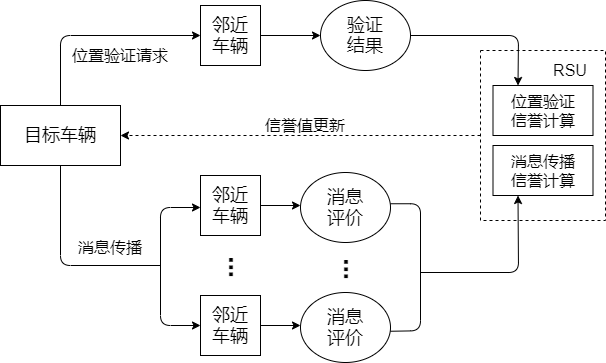
\includegraphics[width=0.8\linewidth]{figures/model.png}
  \caption{信誉评估算法交互模型示意图}
  \label{fig:model}
\end{figure}

\begin{figure}
  \centering
  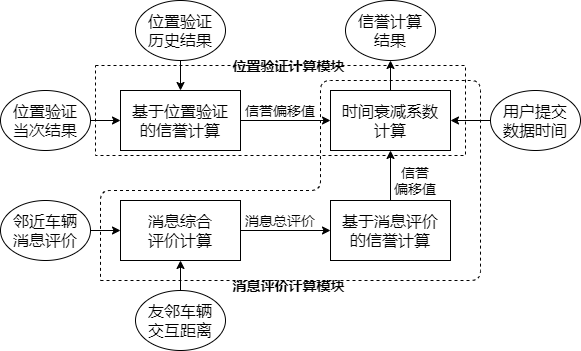
\includegraphics[width=0.8\linewidth]{figures/algo.png}
  \caption{信誉评估算法流程图}
  \label{fig:algo}
\end{figure}

\section{信誉计算方式}

本节将介绍车辆信誉算法涉及到的具体公式。将目标车辆的信誉值记为$T$,$T$是在$[0,100]$范围内的整数。在目标车辆作为新用户加入到车载网中时,它被赋予初始信誉值$T_0$。每次进行位置验证或消息传播后,车辆间交互的结果将被用于计算目标车辆新的信誉值$T'$。下面介绍信誉值更新的具体算法。

\subsection{时间衰减系数}
目标车辆基于一次交互更新的信誉值为:

\begin{equation}
    T'=T+\Delta T*D(t)
    \label{eq:credit}
\end{equation}

其中$T$为本次信誉计算前车辆的原始信誉值,$\Delta T$为根据本次交互结果计算得到的信誉偏移值,$D(t)$表示基于数据提交时间间隔得到的时间衰减系数,其计算方法如下:

\begin{equation}
    D(t)=\frac{1}{\delta*(t-t_l)}
    \label{eq:timedecay}
\end{equation}

其中$\delta$为参数,$t$表示本次提交数据的时间,$t_l$表示上一次提交数据的时间。通过公式\eqref{eq:timedecay}引入时间衰减系数,目的在于以数据提交时间间隔对用户活跃度进行量化。在公式\eqref{eq:credit}中将信誉偏移值与时间衰减系数进行叠加,使得活跃度这一指标在信誉调整的幅度上能够得到明确的体现,而同时避免了交互结果对信誉的影响被完全覆盖:成功的交互必然能导致信誉提升,失败的交互必然能导致信誉下降,但是交互的频率作用于信誉的增减幅度,长时间不提交数据会导致一次交互结果对信誉值的总影响减弱。

\subsection{基于位置验证的信誉计算}
在目标车辆进行一次位置验证之后,其信誉偏移值的计算方式如下:

\begin{equation}
    \Delta T=\left\{\begin{aligned}
    &max(\theta_{s}*(sRate+1)+\theta_{f}*fRate,0), & \mbox{本次验证成功}\\
    &min(\theta_{s}*sRate+\theta_{f}*(fRate+1),0), & \mbox{本次验证失败}\\
    \end{aligned} \right.
    \label{eq:locproof}
\end{equation}

其中$sRate$、$fRate$分别表示目标车辆在近期一段行驶历史中位置验证的成功率和失败率。该公式保证了本次验证结果对信誉偏移方向的决定性影响:本次验证成功必然使信誉提升,本次验证失败必然使信誉下降。除了对当次位置验证结果进行考量之外,\eqref{eq:locproof}还引入了历史记录中的验证结果,在保证本次验证占有最大权重的同时对信誉偏移的计算结果进行平滑处理。

\subsection{基于消息传播的信誉计算}
在目标车辆i向周围车辆发送一条消息m之后,收到这条消息的邻近车辆j将根据消息内容的准确性对其进行打分,分数$R_j^m$为$[1,10]$之间的整数。在汇总了所有周围车辆对消息m的打分之后,可计算其总评价:
\begin{equation}
    Cred_m=\frac{\sum_jw_{ij}*R_j^m}{\sum_jw_{ij}}
    \label{eq:messagecred}
\end{equation}

其中权重$w_{ij}$由车辆$i$、$j$的距离$dis(i,j)$决定:
\begin{equation}
    w_{ij}=e^{-\gamma* dis(i,j)}
    \label{eq:disweight}
\end{equation}

在公式\eqref{eq:messagecred}中,对邻近车辆的打分进行加权的意义在于,邻近车辆对消息内容的评价应当基于自己对实际情况的观察,因此其评价与自身和消息相关事件之间的距离也有一定关系。考虑到这条消息描述的是目标车辆所处位置的事件,故可用目标车辆和邻近车辆之间的距离表示消息描述事件和消息评价者之间的距离。从公式\eqref{eq:disweight}中可以看出,两辆车距离越近,对应的消息打分所占权重越高,代表该邻近车辆对事件的观察、对消息的评价更具有说服力。

在计算得到消息m的总评价后,可根据$Cred_m$判定消息是否可信,从而计算相应的信誉偏移值:

\begin{equation}
    \Delta T=\left\{\begin{aligned}
    &Reward=\alpha*D*\frac{1}{e^L}, &{Cred_m\geq C_0,\mbox{消息可信}}\\
    &Punishment=(-1)*\beta*D*\frac{1}{e^L}, & {Cred_m<C_0,\mbox{消息不可信}}\\
    \end{aligned} \right.
    \label{eq:message}
\end{equation}

其中$C_0$为参数,$D$表示车辆密度,$L$表示消息的紧急级别($L=1$:事故警告;$L=2$:路况提示)。可以看到,车辆密度越大、消息内容越紧急,计算得到的信誉偏移幅度就越大,因为有更多的车辆受到了这条消息的影响。

\section{科学性分析}

当车辆在道路上正常行驶,并能够持续、稳定地与周围车辆完成交互时,该算法显然能保证目标车辆信誉值的稳步上升;然而实际应用中,可能会遇到各种特殊情况,不论是否是人为制造,都会导致车辆交互失败并使其信誉值下降。本节将针对一些可能出现的意外情况进行具体讨论,分析上文提出的算法是否能在这些情况下合理、公正地体现车辆信誉的变化。

\begin{enumerate}
    \item 客观原因导致交互失败。目标车辆可能由于自身设备出现故障等原因,导致无法获取准确的地理位置信息,或者中断与其他车辆的通讯,进而导致信誉值的下降。这种情况的出现,并不违背本文算法设计的前提:车辆信誉值是为其他车辆提供的、用于判断该车辆提供信息是否可信的评价指标,即使是由于客观原因导致的交互失败,也意味着目标车辆当前的状况并不适合与其他车辆共享信息。对于个别偶然的失败情况来说,本文算法引入了历史记录进行偏移值的平滑,这使得拥有良好交互记录的车辆不会大幅损失信誉值;如果在一段时间内存在持续的失败交互,车辆的信誉值将降低至不可信水平,但是如果影响车辆的客观因素消失,其信誉值还能够通过之后的正常活动重新回升。
    \item 恶意诋毁。道路上可能存在一些恶意的车辆,在作为邻近车辆参与交互时故意给予负面的反馈,譬如声称其他车辆位置验证请求中的地理信息不合法,或者故意给其他车辆发出的消息打出低分。本文算法没有为了避免这种情况而进行专门的设计,但是可以看到当这种恶意车辆在整体交通中仅占少数部分时,它们的诋毁行为不会对诚实车辆的信誉产生明显的影响。对于位置验证,考虑到历史验证成功率对整体结果的平滑,个别的验证失败结果对车辆可信度影响不大。对于消息传播,消息总评价由多车打分的加权平均得到,并且最终只通过消息是否可信来判定信誉值增减,而不考虑可信范围内具体的分数高低。因此,少数的恶意负面评价通常也很难影响最后的整体结果。
    \item 多人合谋。车载网系统中还可能面临的一种安全威胁,是多台恶意车辆之间的合谋,例如一台恶意车辆可以发送包含虚假位置信息的位置验证请求,而其合谋者为其提供捏造的确认信息,两者通过这种形式完成了一次成功的位置验证并获得了信誉值的提升,尽管验证的信息实际上并不合法。对于本文提出的算法来说,这种形式的攻击仅当与之合谋的车辆足够多时才能够收获明显的效果。这是因为区块链上维护了一段时间内的车辆交互结果记录,而同一对车辆在这段时间内不能反复地进行同样的交互。如果其他车辆能够正常地识别恶意车辆信息的异常,那么这种合谋行为也难以有效地提升其信誉值,除非周围的车辆都是与之串通的共犯;但是在实际情况中,这样做的伪造成本会变得极其高昂,再考虑到车辆的流动,其可行性也是较低的。
\end{enumerate}

\section{本章小结}
本章介绍了对车辆信誉进行计算时所考量的因素以及具体的计算公式,并通过一些可能出现的实际情况分析了算法的合理性与科学性。算法主要依靠车辆之间交互的结果确定信誉的增减,包括位置验证和消息传播两部分;其中,对位置验证结果的计算中引入了历史验证成功率进行结果的平滑,对消息评价的计算中考虑了交互车辆之间的距离对评价权重的影响。同时,算法引入了引入了时间衰减系数,根据活跃度调整信誉增减的幅度。最后,本章分析了该算法的科学性与稳定性,对于可能的意外故障或潜在的恶意攻击,该算法都能较好地通过信誉值反映车辆当前的实际状况。
\chapter{信誉评估算法原型系统的实现}

本章对车辆信誉评估算法的原型系统进行了详细的介绍。该系统主要由浏览器端和智能合约端两部分构成。浏览器端主要进行车辆行驶数据获取、车辆交互模拟以及行驶状态的可视化展示,智能合约端负责数据的存储以及车辆信誉评估算法的具体实现。原型系统的整体架构如图~\ref{fig:proto}所示。

\begin{figure}
  \centering
  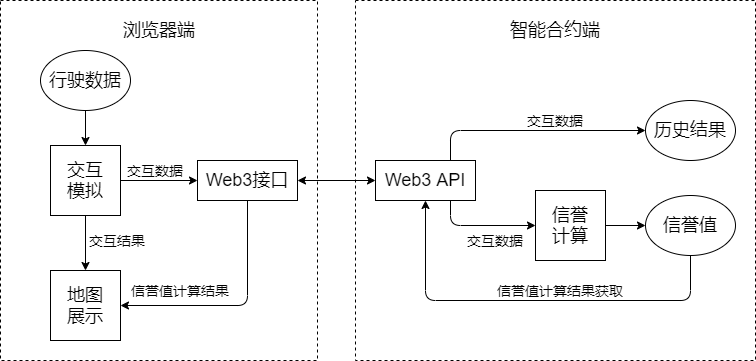
\includegraphics[width=0.8\linewidth]{figures/proto.png}
  \caption{车辆信誉评估原型系统架构图}
  \label{fig:proto}
\end{figure}

\section{总体框架及运行环境}
信誉评估算法的原型系统框架主要分为两个部分:浏览器端及智能合约端。浏览器端模拟实际场景中的车辆终端,进行位置信息获取、车辆交互等数据处理任务;智能合约端模拟实际场景中的路侧单元(RSU),对车辆的信誉进行更新和维护。考虑到智能合约对于复杂运算存在较大的限制,同时区块链上的大量计算需要付出相应的执行费用,因此该原型系统中位置验证、消息传播的模拟由浏览器端负责,将模拟的交互结果上传至区块链后,合约端仅负责信誉值的评估计算。本原型系统的运行流程如下:
\begin{enumerate}
    \item 系统初始化。浏览器端通过web3.js接口对信誉评估的智能合约进行初始化,同时加载地图和车辆行驶的道路数据,转化为Geohash格式存储,便于之后的合约计算。结合加载的缓存数据,为目标车辆生成用户的通用唯一识别码,作为该车辆身份的确认证明,此后浏览器端将对该目标车辆的行驶路线和信誉值变化进行追踪。
    \item 模拟车辆交互。车辆交互结果的模拟是浏览器端的重要部分,该步骤中程序对目标车辆和其行驶途中遇到的邻近车辆分别进行位置验证和消息传播的模拟,并最终给出模拟交互的结果。具体实现方式见3.2节。
    \item 上传交互结果。获得交互结果(位置验证结果或者邻近车辆给出的消息评价)之后,浏览器端利用web3.js接口将该结果的相关数据打包上传至区块链,在合约端进行结果数据的存储,并进行信誉值计算。
    \item 信誉评估。信誉评估是合约端程序的主要内容,依据模拟交互的结果、数据上传的时间及上一章中设计的算法进行信誉值的计算和更新。针对智能合约在计算开销方面的限制,笔者在信誉评估合约中采取了一系列简化计算的措施,具体情况见3.3节。
    \item 地图展示。浏览器端使用了leaflet(一个开源的JavaScript互动地图库,适用于移动设备)\cite{leaflet}进行地图及车辆行驶路线的展示。在合约端完成信誉值的更新之后,浏览器端可以通过web3.js接口获取更新之后的信誉值,该信誉值及本次车辆交互的结果都可以在leaflet地图中得到可视化展示,具体情况见3.4节。
\end{enumerate}

本章中的系统在Ubuntu 20.04操作系统中实现,使用Solidity v0.8.0实现智能合约,并通过Web3.js v1.2.9实现浏览器端功能,以及与以太坊区块链的对接。在系统开发及测试过程中,使用Truffle v5.1.62进行智能合约的编译与本地私有链的部署,同时结合私有链的可视化工具Ganache v6.12.2进行便利的调试与开发。

\section{车辆交互模拟}
该原型系统中,浏览器端负责车辆交互的模拟,其中包括位置验证的模拟和消息传播的模拟。对于位置验证,每次模拟只涉及到目标车辆和一台邻近车辆;对于消息传播,每次交互(即同一条消息的发送与评价)涉及到目标车辆及其周围的多方车辆。在程序中两种场景的模拟独立进行,分别选取对应的参与车辆并各自进行交互的模拟,两者的结果互不影响。下面,文章将分别介绍两种交互的具体模拟形式。
\subsection{位置验证模拟}
在目标车辆行驶过程中,它可以向一定范围内的邻近车辆发送请求,表明希望他人为自己提供位置验证,当一辆邻近车辆收到该请求后,可以视为两辆车进行了一次位置验证的交互,而最终是否获取有效的位置验证即为本次交互结果成功或失败的判断标准。在实际情况中,位置验证是否成功可能取决于以下因素:参与交互的车辆对当前行驶区域的熟悉程度;交互车辆获取地理位置信息的准确度;交互车辆之间的通讯信号强度;交互车辆中是否存在恶意行为。

在本文所实现的原型系统中,对位置验证过程中通信的具体内容不做过多考虑,仅通过上述影响因素模拟位置验证的结果,具体思路如下:
\begin{enumerate}
    \item 对于目标车辆当前所处区域(在该原型系统中,区域按照具体的城市道路进行划分),在每个区域中,根据目标车辆历史记录中对该区域的到访情况,即车辆对该区域的熟悉程度,该车辆拥有一个位置验证成功率的基准波动范围。目标车辆经常行驶的区域,对应的基准范围相对更高;对于不够熟悉或者未曾到访过的区域,对应的基准范围相对较低。
    \item 目标车辆与邻近车辆进行一次位置验证交互时,其成功率在上述基准范围之内波动,并最终由两辆车之间的交互距离所确定。其中,交互距离为两辆车在行驶途中所能达到的最短距离,该距离与位置验证的成功率成一次负相关关系。
    \item 在确定了当次位置验证的成功率之后,程序通过伪随机数模拟得到最终的位置验证结果为成功还是失败,并将该结果及相关数据上传至合约端。
    \item 特别地,在参数测试与评估阶段,为了有针对性地研究特定环境下各参数取值对应的特征,部分测试中略去了行驶道路和交互距离对验证成功率的影响,仅通过伪随机数模拟来观察在确定的验证成功率条件下,不同参数取值对系统的影响。
\end{enumerate}

\subsection{消息传播模拟}

在特定事件(比如道路拥堵、交通事故等)发生时,目标车辆可以向邻近车辆发送消息,告知自己观察到的事件信息。由于特殊事件的发生属于偶然情况,因此消息传播这一交互行为的频率相对较小,并且每次仅对一定范围内的特定车辆群体有效。邻近车辆对消息内容的评价和自身与实际事件发生位置之间的距离相关,在本系统中使用该车辆与目标车辆之间的距离进行替代。

与位置验证类似,在程序实现中笔者同样忽略具体的事件及消息内容,主要对接收消息的车辆群体及它们给出的消息反馈进行模拟,主要流程如下:
\begin{enumerate}
    \item 确定接收消息的邻近车辆。以目标车辆为中心,取与之相距在五个单位之内的所有车辆,为接收到本次交互消息并给出评价的车辆群体。在模拟测试中,周边车辆沿道路呈区域性的均匀分布(车辆密度不同);在实际测试中,周边车辆的分布则完全由真实数据决定。
    \item 模拟邻近车辆的消息评价。每台收到消息的车辆给出对消息的打分,分数是$[1,10]$之间的整数。在参数测试阶段,为了对距离衰减系数$\gamma$的取值进行评估,并对消息总评价进行可信区域划分,该部分选取了几种消息评价的分布情况,分别进行模拟:评价分数在$[1,10]$之间完全随机;与目标车辆距离较近的中心车辆给出的分数和边缘车辆相差较大(中心车辆评价大于5分、边缘车辆评价小于5分,或者相反情况)。
    \item 在浏览器端收集各邻近车辆给出的消息评分,并预先计算每辆车与目标车辆之间的距离,保证评分与交互距离一一对应,并将数据打包上传至合约端。
\end{enumerate}

\section{信誉评估智能合约}

智能合约中实现了第2章中的信誉评估算法,并进行相关数据的存储,在实际应用中对应路侧单元(RSU)的功能。由于合约部署在区块链上,具有公开透明、可追溯等特点,因此为信誉计算提供了安全性的保障,从底层结构上确保这一过程是具有权威性的,避免了对信誉值可能的篡改行为。

在本文实现的合约中,以用户为单位进行数据的维护,通过通用唯一识别码(UUID)与用户信息的数据结构user建立映射。在用户信息中,主要维护的数据内容包括历史数据提交时间、位置验证的历史结果统计、用户信誉值等。除此之外,合约中还实现了message数据结构,用于消息传播发生时的信誉计算,其中维护消息发送者UUID、各车辆给出的消息评分、各车辆与消息发送者之间的距离等。

当且仅当目标车辆与邻近车辆完成一次交互模拟之后,浏览器端会上传相应的数据并调用合约中信誉计算的相关接口;合约端则根据交互类型,选择进行位置验证或消息传播结果的数据处理,并进一步完成信誉值的更新。

由于智能合约端的每次计算都会消耗一定的gas(执行开销),同时对内存访问和复杂的数学函数都具有一定的限制,因此合约实现的难点之一就在于在原有算法的基础上对合约计算进行尽可能的简化,采用的具体措施包括:

\begin{enumerate}
    \item 使用Geohash存储地理位置信息。Geohash是一种地理编码系统,它将传统的经纬度位置信息转换为一维的字符串,每个字符串对应一块矩形的地理区域\cite{lwq}。使用这种方式存储位置信息,可以在精度允许的范围内对车辆进行定位,同时将与距离相关的计算过程和结果全部转移到整数范畴中,相比于利用经纬度计算得到了大幅度的精简。
    \item 在浏览器端进行数据预处理。为了节省合约端的计算开销,部分不与信誉值直接相关的数据可以在浏览器端提前进行计算,比如消息传播过程中各车与目标车辆之间的距离,而在合约端只保留信誉计算的核心步骤。
    \item 简化参数相关的计算过程。对于合约端较为复杂的计算步骤,可以事先计算出中间结果,将中间结果作为实际计算的参数。譬如消息传播中涉及到的指数计算,由于系统实现中$dis(i,j)$的实际取值仅限于$[0,5]$之间的整数,因此在参数$\gamma$确定后可直接计算得到几种可能的幂值并将其作为参数写入程序中,在信誉计算的过程中根据距离直接获取相应的中间值即可。
\end{enumerate}

\section{地图展示}
本章使用了OpenStreetMap(OSM)\cite{osm}提供的开源地图获取北京市的道路信息,并利用osm2pgrouting\cite{pg}转换工具提取出道路数据信息进行存储。在原型系统的浏览器端,本章使用leaflet地图组件加载离线OSM数据,并在地图上进行车辆行驶数据、友邻交互以及信誉评估结果的可视化展示。地图中的具体展示内容主要包括以下三项:
\begin{enumerate}
    \item 目标车辆的行驶轨迹。根据目标车辆提供的位置信息,浏览器端在地图上进行数据点的绘制,并最终构成一条完整的车辆行驶轨迹。
    \item 目标车辆与邻近车辆的交互结果。当浏览器端发生一次车辆间的模拟交互时,地图组件将绘制参与交互的邻近车辆此时所在的位置,并通过具体的数据点颜色体现本次交互的模拟结果。
    \item 目标车辆的实时信誉。在绘制目标车辆的行驶轨迹时,每个数据点的颜色代表了车辆此时对应的信誉值评估结果。浏览器端通过web3.js接口从合约端获取更新后的信誉值,并据此选择对应的中间梯度颜色绘制数据点。
\end{enumerate}
本文将在第5章中对地图展示的实际效果与表现含义做进一步的说明。

\section{本章小结}
本章介绍了车辆信誉评估算法原型系统的具体实现。该系统在浏览器端进行车辆交互的结果模拟以及行驶状态的可视化展示,在合约端完成数据存储以及车辆信誉评估算法的实现,通过区块链保证了信誉计算的安全性与可靠性。同时,为了解决智能合约对于复杂数学计算的限制,系统在合约编写方面对具体计算方式进行了一系列优化措施。
\chapter{信誉算法的参数调优与特征分析}
本章使用上述原型系统,针对信誉算法各项参数取值对于系统敏感度、精确度的影响设计了实验。实验对车辆行驶场景进行简化与模拟,通过构造多种不同情况下的交通状态与车辆交互结果,完成对信誉评估算法中各项参数的特征分析和结果调优。

\section{测试方法}
在本节的模拟测试中,笔者将实际交通地形与车辆行驶状况进行了简化,构造沿经线或纬线分布、长度一致、呈田字格式排列的道路,使模拟的目标车辆在道路上匀速行驶,并以相同的时间间隔更新自己的位置信息。

在下文所述的模拟实验中,目标车辆每隔1秒种更新一次自己的位置,走完田字格道路的一条单位边共需100秒,即一条道路上均匀分布行驶轨迹的100个数据点。生成的原始数据点坐标由经纬度表示,经过转换计算可知,两个相邻数据点之间间隔约为10米;在以下实验中,为便于计算与表述,称该长度为单位距离,称田字格道路的一条单位边为一条道路。

因为该实验只对目标车辆的信誉变化进行追踪,因此在邻居车辆的模拟数据生成时,仅生成两辆车交互成功时邻居车辆的坐标点,而不对其进行动态的轨迹模拟。

\section{参数设计与分析}
本节将根据模拟测试的结果,对第2章中信誉算法的各个参数取值进行调优,主要评价内容及分析指标如表~\ref{tab:params}所示。

\begin{table}
  \centering
  \caption{测试参数及评价指标}
  \begin{tabular}{ll}
    \toprule
    测试参数          & 评价指标                         \\
    \midrule
    时间衰减系数的缩放参数$\delta$   & 信誉变化敏感度 \\
    位置验证权重参数$\theta_s$、$\theta_f$   & 信誉变化趋势、对错误结果的敏感度                     \\
    消息传播的距离衰减系数$\gamma$、消息可信区域划分   &    评价结果波动性    \\
    \bottomrule
  \end{tabular}
  \label{tab:params}
\end{table}

\subsection{时间衰减参数}
本实验基于真实的交通状况,对道路上的车辆分布进行了两种模拟:在一条道路上车辆均匀分布,或者在道路的前半部分均匀、相对稀疏地分布,在靠近道路末尾处车辆密集分布。两种情况分别模拟了车辆正常行驶以及在路口处进行等待两种情况。具体地,两种模拟情况中一条道路上都有20台邻近车辆,其中正常行驶情况下20辆车在道路上呈随机、均匀分布,路口等待情况下10辆车在道路前80\%部分随机分布、10辆车在后20\%部分随机分布。

图~\ref{fig:decay}展示了时间衰减系数的缩放参数$\delta$在不同取值下,目标车辆在一条道路上完成随机生成的20次位置验证所对应的信誉曲线变化。其中,各组实验的位置验证总成功率均为80\%,每张子图中的两条曲线分别对应车辆均匀分布、路口处密集分布两种情况。

\begin{figure}
  \centering
  \subcaptionbox{$\delta=0.1$\label{fig:decay01}}
    {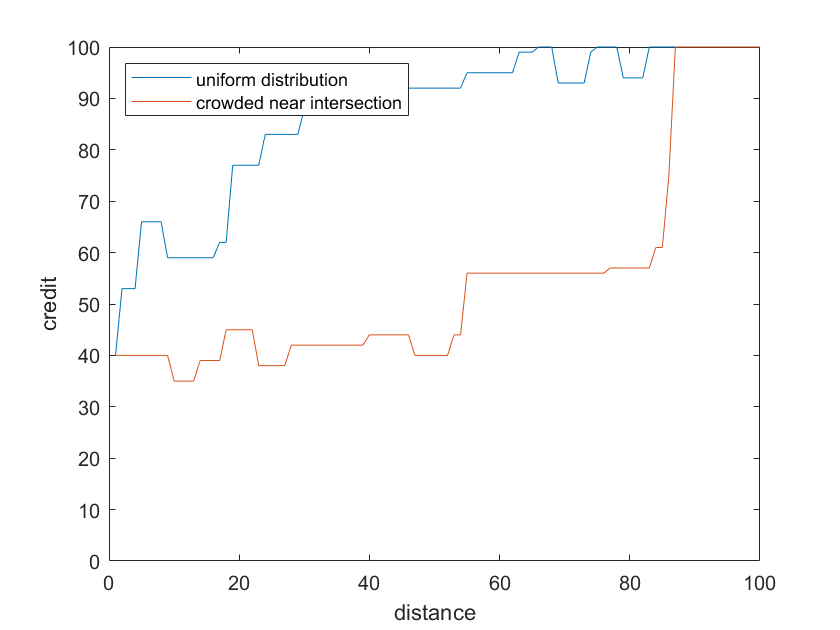
\includegraphics[width=0.49\linewidth]{figures/decay01.png}}
  \subcaptionbox{$\delta=0.2$\label{fig:decay02}}
    {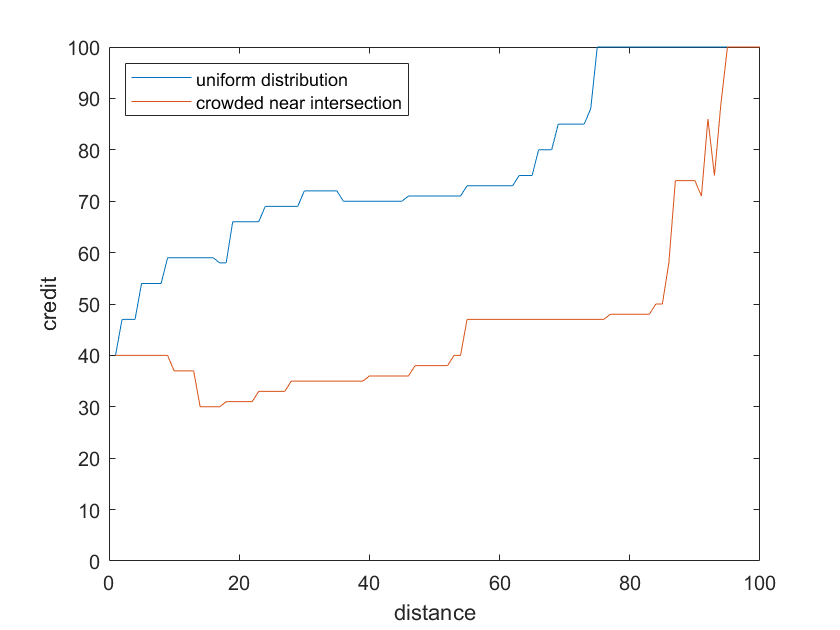
\includegraphics[width=0.49\linewidth]{figures/decay02.png}}
    \subcaptionbox{$\delta=0.3$\label{fig:decay03}}
    {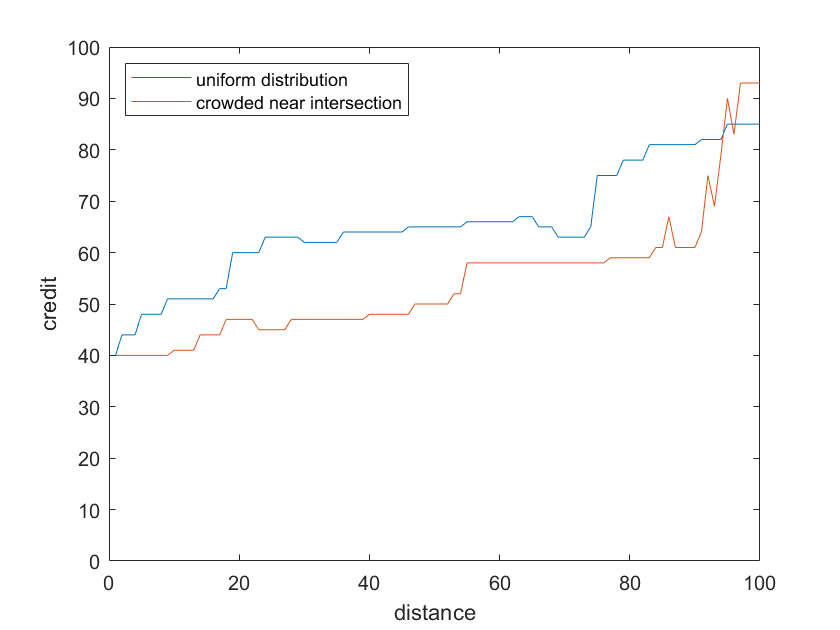
\includegraphics[width=0.49\linewidth]{figures/decay03.png}}
    \subcaptionbox{$\delta=0.5$\label{fig:decay05}}
    {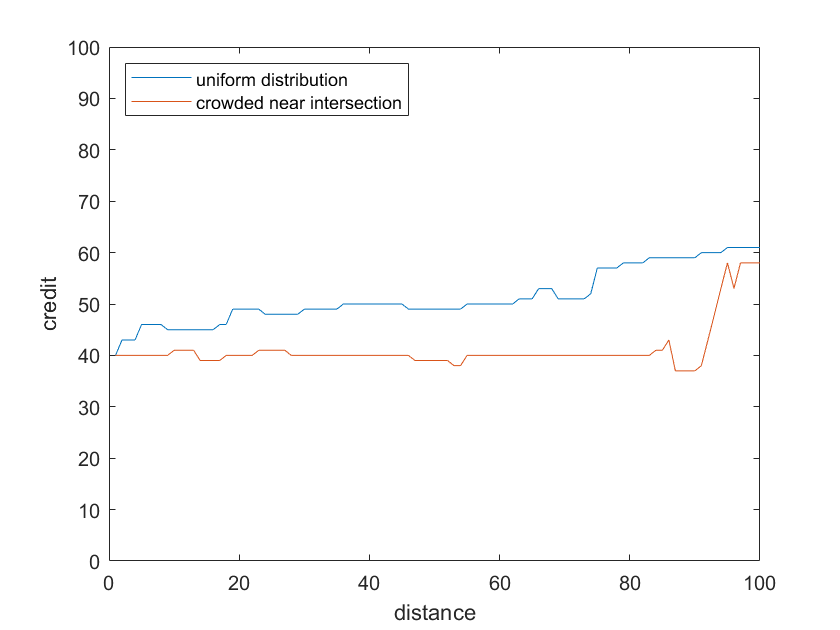
\includegraphics[width=0.49\linewidth]{figures/decay05.png}}
  \caption{不同$\delta$值在两种车辆分布模式下的信誉曲线}
  \label{fig:decay}
\end{figure}

可以看到,在位置验证成功率较高的条件下,各组实验中目标车辆的信誉曲线基本都呈上升趋势,但是数值的波动对数据提交时间的敏感度相差很大;尤其是当有多辆车在路口处密集分布时,过小的缩放参数与频繁的数据提交非常容易导致信誉值的暴涨或暴跌,而这一现象可能只需要两到三次集中的位置验证结果就能发生。相反地,同样可以看到,当该缩放参数取值过大时,目标车辆在正常行驶的过程中则很难产生足够明显的信誉值变化,必须依靠足够密集的数据才能使其得到实质上的提升。该结果一部分是由于智能合约上对数据计算的限制,系统最终会将信誉偏移值归约为整数,如果对数据提交时间的缩放系数不够小,该计算结果很容易会被削减至0,使得交互结果对信誉的影响完全得不到体现。

图~\ref{fig:decay_comp}更加明显地体现了参数$\delta$的取值对系统敏感度的影响。本组实验选取了不同的位置验证成功率和邻近车辆分布,对于每种情况都随机生成同一组交互结果,每个子图展示了在该组交互结果下参数不同取值对信誉曲线的影响。可以看到,每组实验中信誉曲线的整体走势基本一致,但是数据增减的幅度差别很大。考虑到需要让系统对交互结果拥有足够的敏感度,同时避免车辆密集的情况下出现极端的波动,经过多次对比试验,确定$\delta=0.2$为合适的缩放值。

\begin{figure}
  \centering
  \subcaptionbox{验证成功率80\%,均匀分布\label{fig:decaye80}}
    {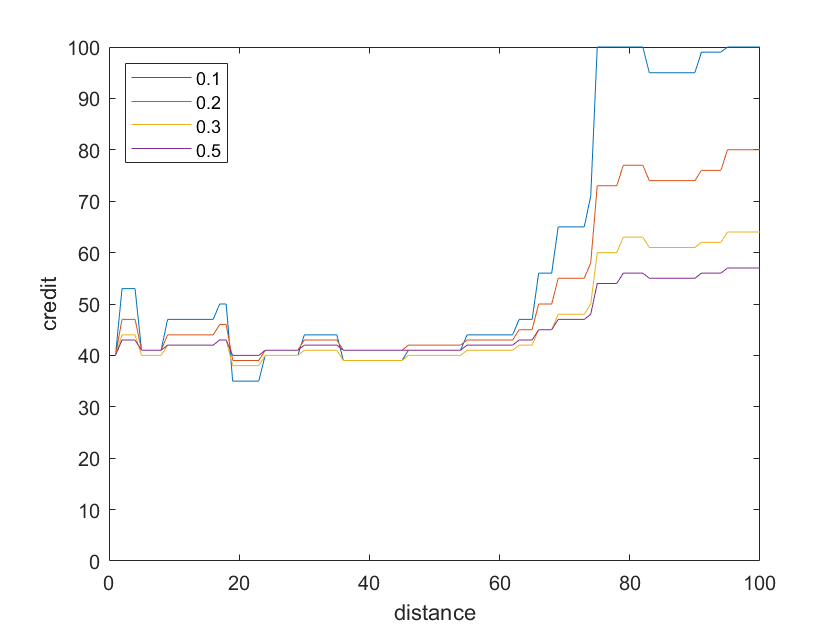
\includegraphics[width=0.49\linewidth]{figures/decay_even_80.png}}
  \subcaptionbox{验证成功率60\%,均匀分布\label{fig:decaye60}}
    {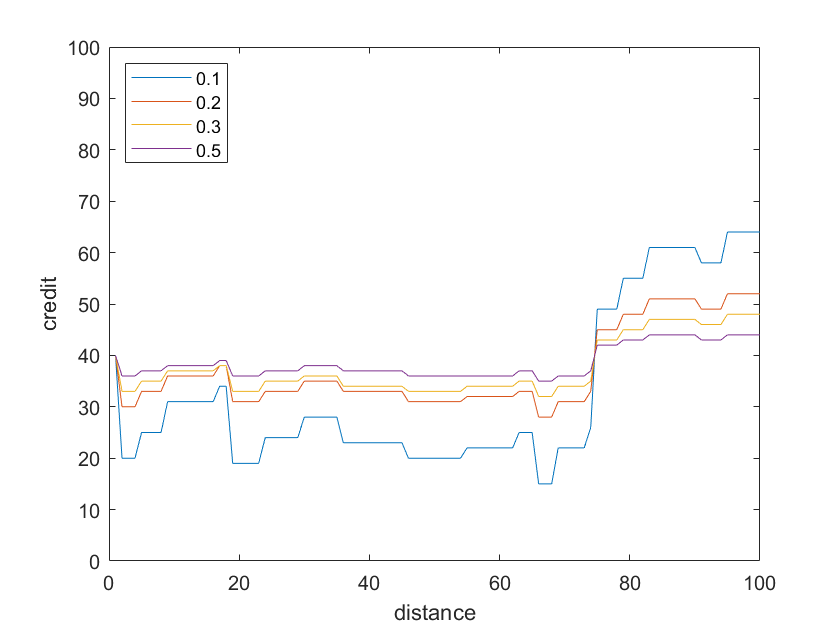
\includegraphics[width=0.49\linewidth]{figures/decay_even_60.png}}
    \subcaptionbox{验证成功率80\%,路口密集\label{fig:decayu80}}
    {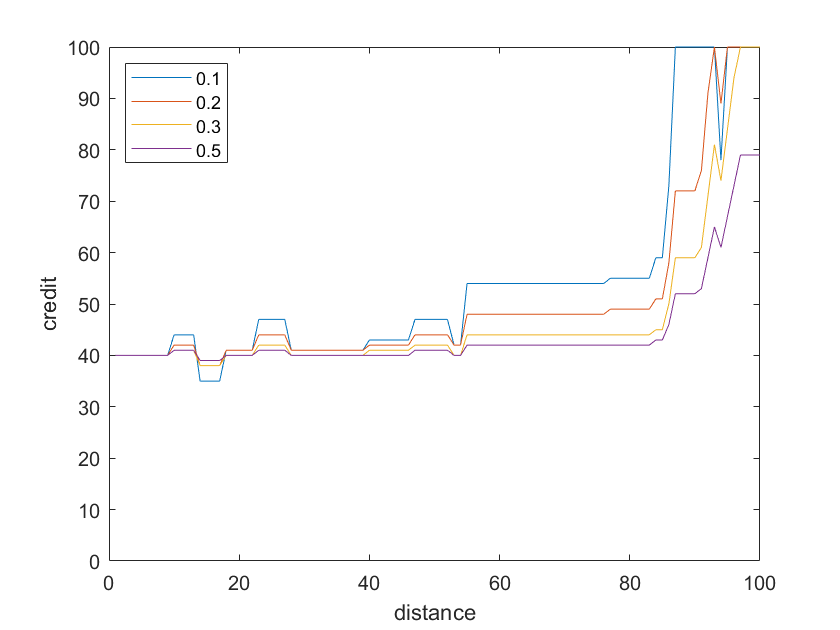
\includegraphics[width=0.49\linewidth]{figures/decay_ueven_80.png}}
    \subcaptionbox{验证成功率60\%,路口密集\label{fig:decayu60}}
    {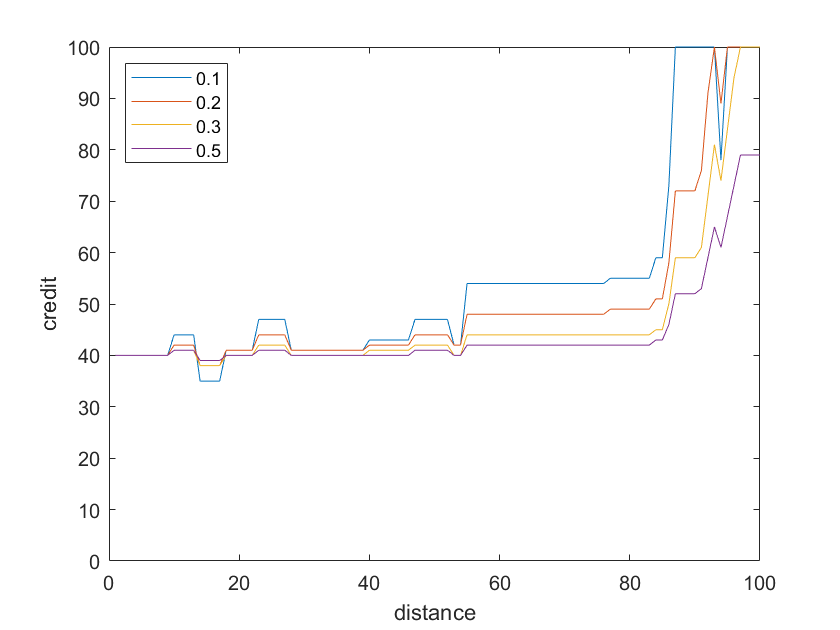
\includegraphics[width=0.49\linewidth]{figures/decay_ueven_80.png}}
  \caption{不同$\delta$值在同一组交互结果下的信誉曲线}
  \label{fig:decay_comp}
\end{figure}

\subsection{基于位置验证的信誉计算参数}
在对位置验证结果的信誉计算中,验证结果成功、失败分别对应一个权重参数$\theta_s$、$\theta_f$。本节的实验中,首先对两参数绝对值的大小关系进行讨论,然后再针对具体取值做进一步的实验。

对于车辆在路口处密集分布的情况,假设总体的位置验证成功率为80\%、60\%、40\%,对这三种场景分别随机生成一组验证结果,具有不同大小关系的权重参数在各组验证结果下所展现的信誉曲线如图4.3所示。三张子图显示的结果相对较为统一,每张图中三条曲线由上至下,对于位置验证失败情况的敏感度依次增强。

值得注意的是,虽然测试中各组参数对每次位置验证结果单独的响应是基本一致的,但是在目标车辆行驶完一条道路后信誉值在整体上的变化有所不同。这一点在图~\ref{fig:theta_comp}b中体现得尤为明显:在位置验证成功率为60\%的情况下,第一组参数对应的曲线最终达到了信誉最大值,但是对于同样的验证结果,第三组参数对应的信誉则基本一直维持在较低的不可信水平。

\begin{figure}
  \centering
  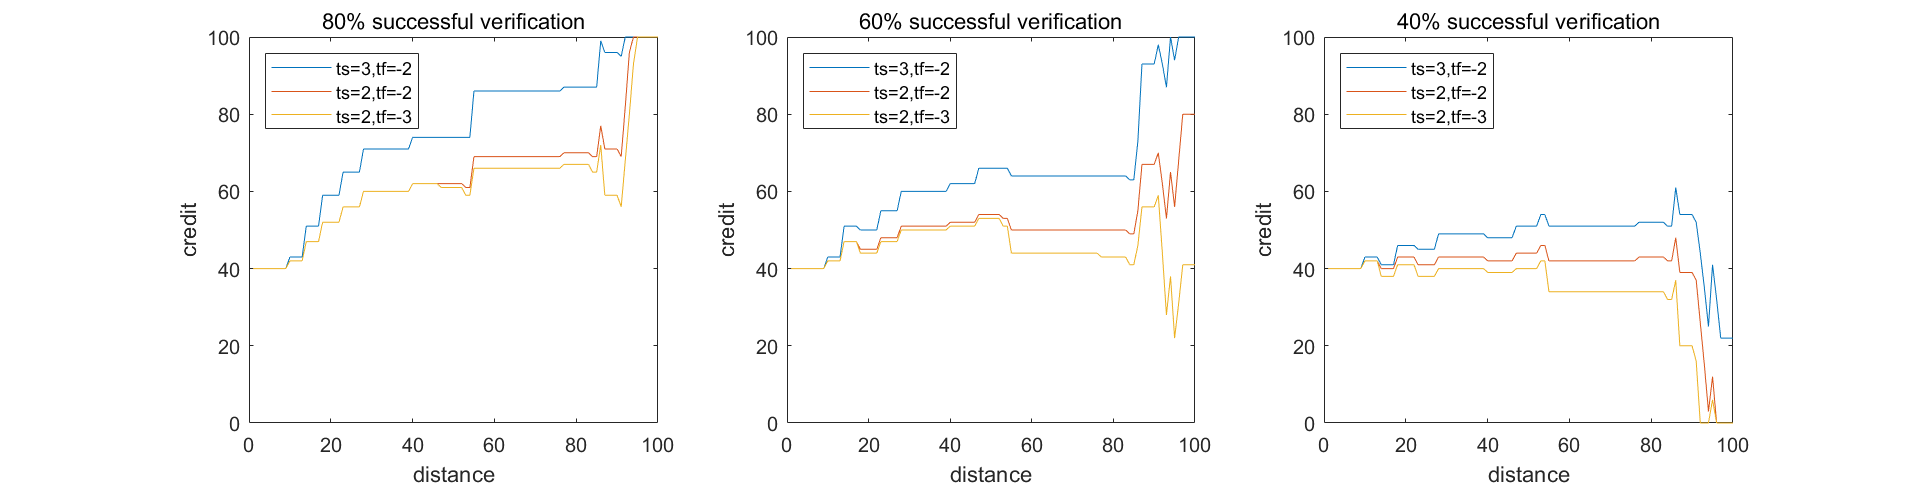
\includegraphics[width=1\linewidth]{figures/theta_comp_total.png}
  \caption{给定验证成功率时,权重参数不同数量关系对应的信誉曲线}
  \label{fig:theta_comp}
\end{figure}

基于上述实验,最终选择两参数的大小关系为$\theta_s<\theta_f$,是考虑到判定一个车辆可信应当需要其在一定程度上持续、稳定地与其他车辆完成成功的位置验证,相对地,验证失败对应的惩罚应当更大,否则仅靠少数成功结果就能很快弥补信誉值的缺失是不合理的。

在确定参数的大小关系后,笔者进一步选取了几组不同的参数取值,重复上述实验。图~\ref{fig:theta_num}展示了各组参数对应的信誉变化结果。通过多次对比实验,最终确定权重参数取值$\theta_{s}=2,\theta_{f}=-3$,使得数据波动能够保持在合理范围内,同时确保每一次计算信誉偏移值时,当次验证结果的影响力能够得到充分的体现,而不被历史数据掩盖。

\begin{figure}
  \centering
  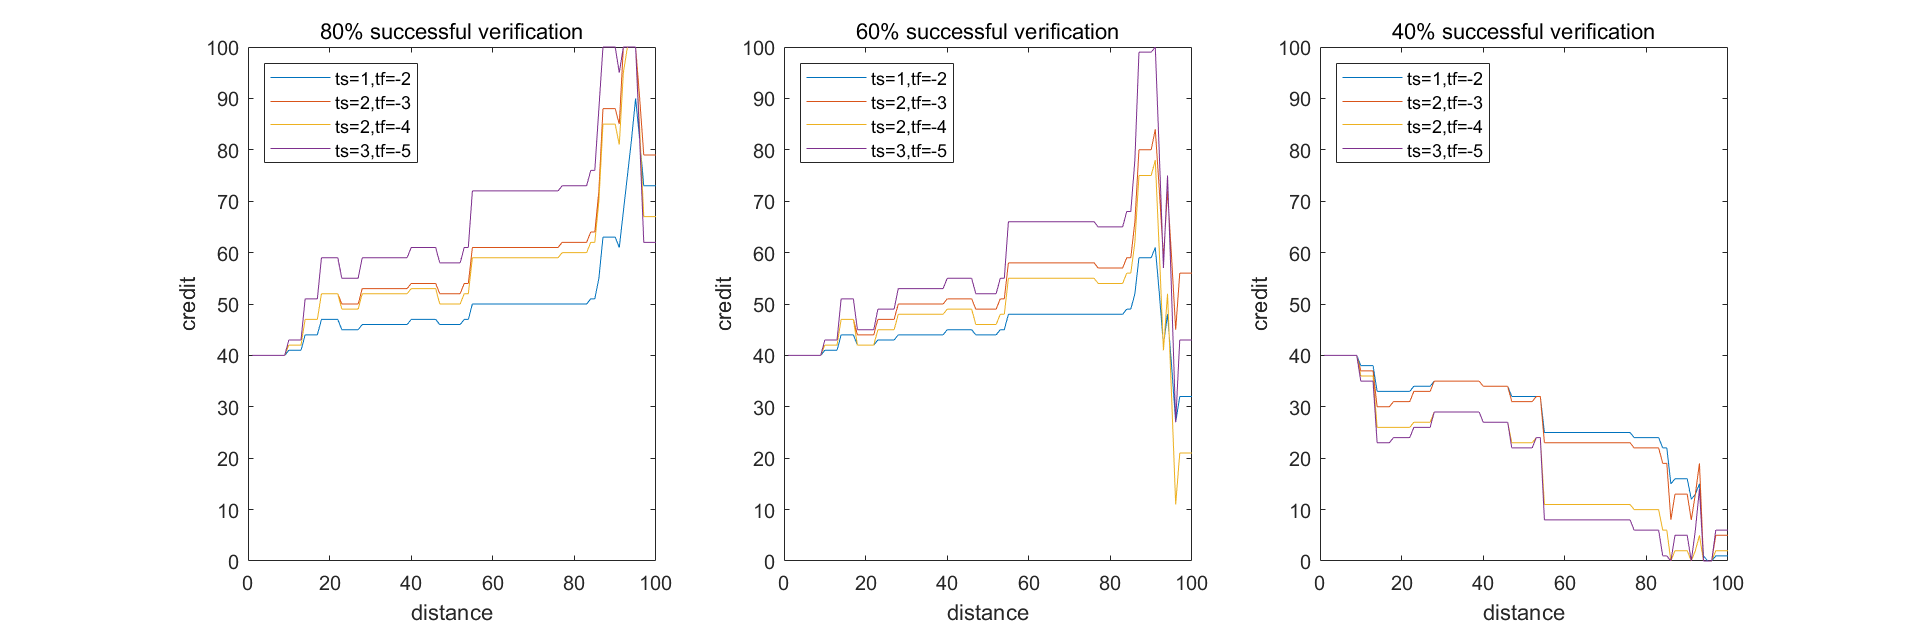
\includegraphics[width=1\linewidth]{figures/theta_num_total.png}
  \caption{给定验证成功率时,权重参数不同取值对应的信誉曲线}
  \label{fig:theta_num}
\end{figure}

\subsection{基于消息传播的信誉计算参数}
本节实验主要研究距离衰减系数$\gamma$对消息总评价的影响,主要通过调整收到消息的邻近车辆数、邻近车辆评价分布情况来确定合适的参数取值。实验中规定与目标车辆相距5个单位距离的车辆为收到消息并给出评价的邻近车辆,该群体的规模在5-15辆车之间;每辆车给出的评价为$[1,10]$之间的整数。同时,为了研究车辆距离与评价分布对总评价的影响,实验进一步规定了,与目标车辆相距2个单位距离及以内的车辆为中心车辆,其余车辆为边缘车辆。实验模拟了三种消息评价的分布模式:所有车辆给出的评价值都在$[1,10]$之间完全随机;中心车辆评价普遍高于边缘车辆(中心车辆打分集中在$[5,10]$,边缘车辆打分集中在$[1,6]$);中心车辆评价普遍低于边缘车辆(中心车辆打分集中在$[1,6]$,边缘车辆打分集中在$[5,10]$)。一次模拟按规则生成交互群体与交互结果,并根据算法计算得到消息的总评价;对于每组确定的邻近车辆数和分布模式,实验重复1000次模拟,记录消息总评价的平均值,结果如图4.5所示。

\begin{figure}
  \centering
  \subcaptionbox{随机评价\label{fig:gammarand}}
    {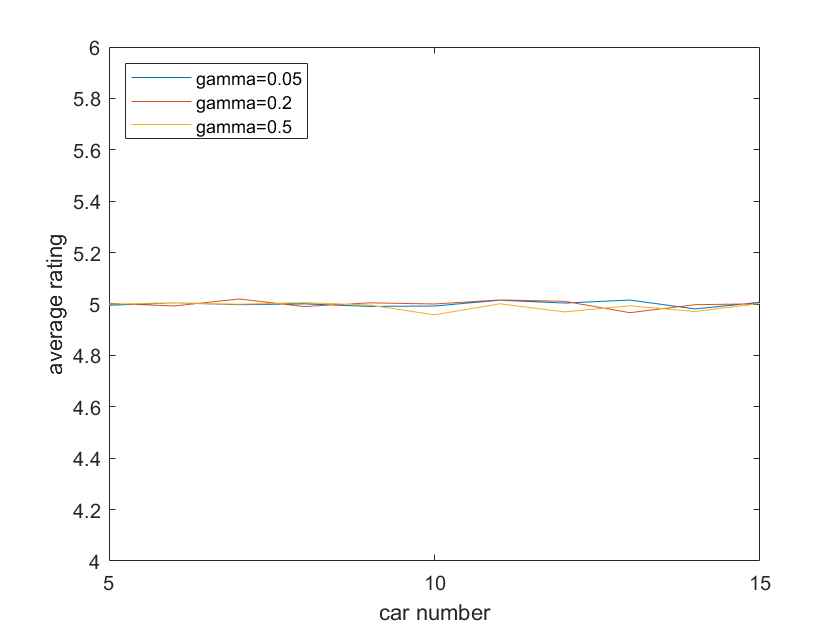
\includegraphics[width=0.49\linewidth]{figures/gamma_random.png}}
  \subcaptionbox{中心评价高于边缘评价\label{fig:gammahi}}
    {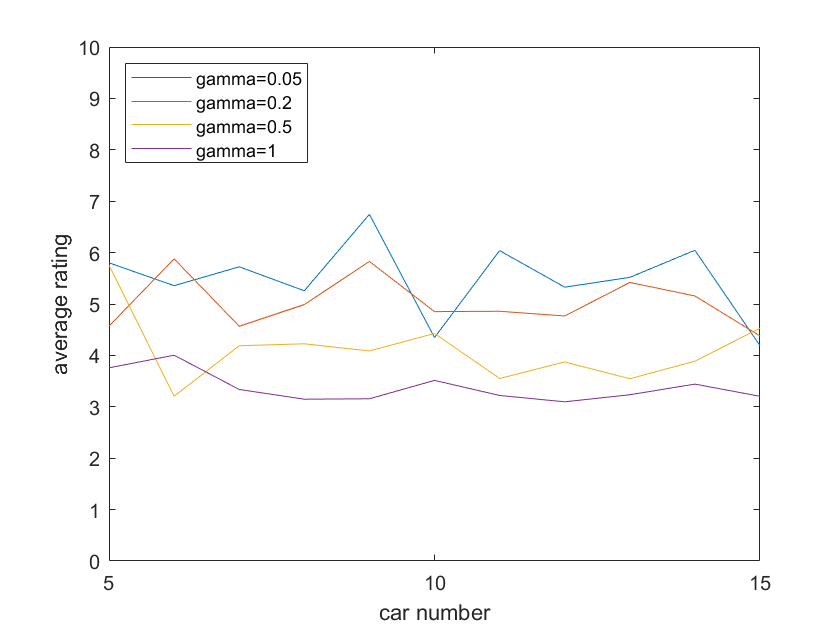
\includegraphics[width=0.49\linewidth]{figures/gamma_centerhi.png}}
    \subcaptionbox{中心评价低于边缘评价\label{fig:gammalo}}
    {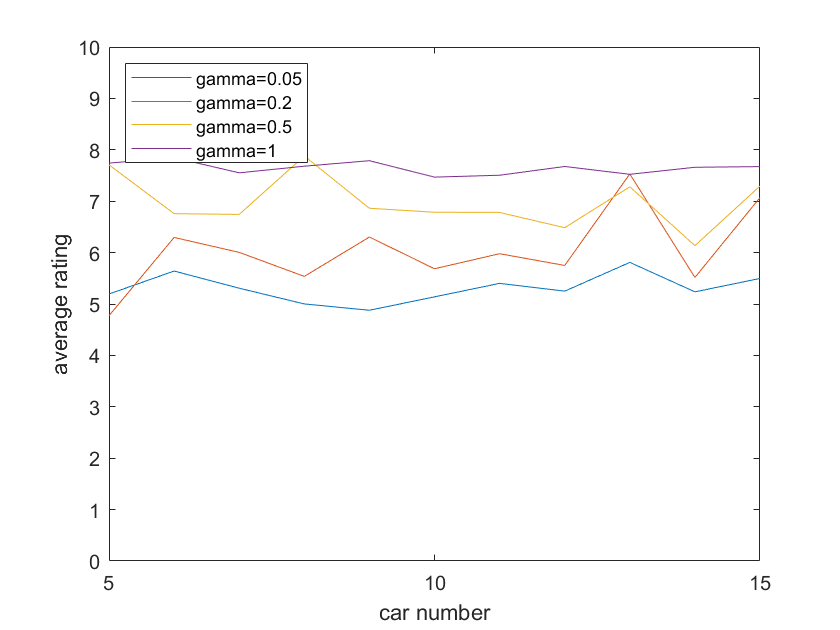
\includegraphics[width=0.49\linewidth]{figures/gamma_centerlo.png}}
  \caption{不同$\gamma$值在三种评价分布模式下对应的消息总评价均值}
  \label{fig:gamma}
\end{figure}

三张子图分别对应三种不同的消息评价分布,每张子图中,横坐标为邻近车辆的数量,纵坐标为消息总评价的均值,不同颜色的曲线分别对应参数$\gamma$的不同取值。从图~\ref{fig:gammarand}可以看出,在评价分布完全随机的情况下,车辆群体大小、$\gamma$取值对消息总评价在整体上几乎没有影响,其均值稳定在5分。图\ref{fig:gammahi}、图\ref{fig:gammalo}中消息评价均值随车辆群体规模的波动相对更大,但也是随机的,可以认为该因素对评价结果没有指向性的影响;同时容易看到,在中心车辆与边缘车辆给出评价相差较大时,$\gamma$取值越小,总评价在整体上就越偏向于中心车辆给出的评价。

图~\ref{fig:gammaerr}展示了后两种评价分布情况下,消息总评价在1000次模拟中的最大最小值。不完全随机的评价导致的数据波动幅度显然比完全随机要更大,$\gamma$取值较大时,周边车辆群体大小导致的数据波动下降,但是对于相同数量的群体来说,极端情况下给出的评价与平均值之间的差距要稍大一些。考虑到车辆距离与评价准确性之间的关系(中心车辆的评价通常来说比外围车辆更有说服力),以及数据的波动、稳定性等因素,选择较小的距离衰减系数$\gamma=0.2$。

\begin{figure}
  \centering
  \subcaptionbox{中心评价高于边缘评价\label{fig:gammahie}}
    {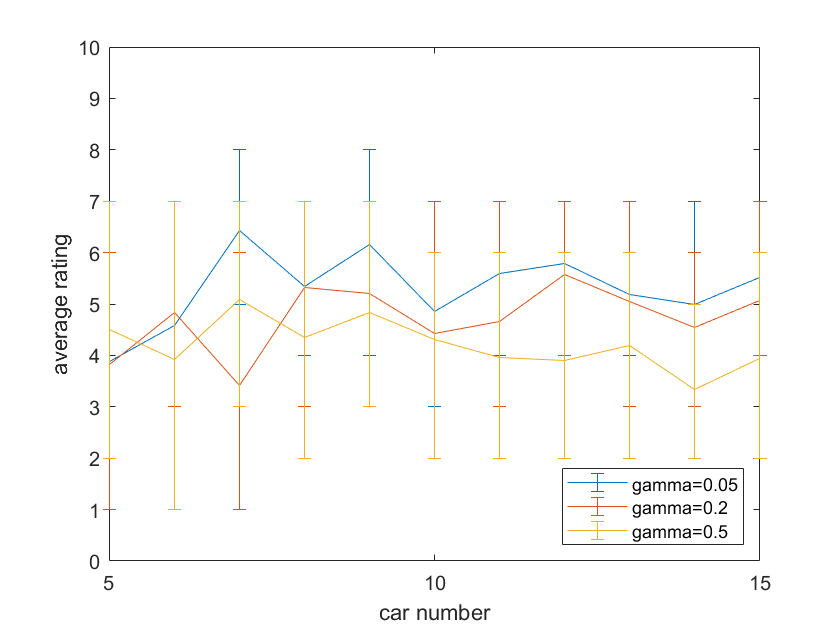
\includegraphics[width=0.49\linewidth]{figures/gamma_centerhi_err.png}}
  \subcaptionbox{中心评价低于边缘评价\label{fig:gammaloe}}
    {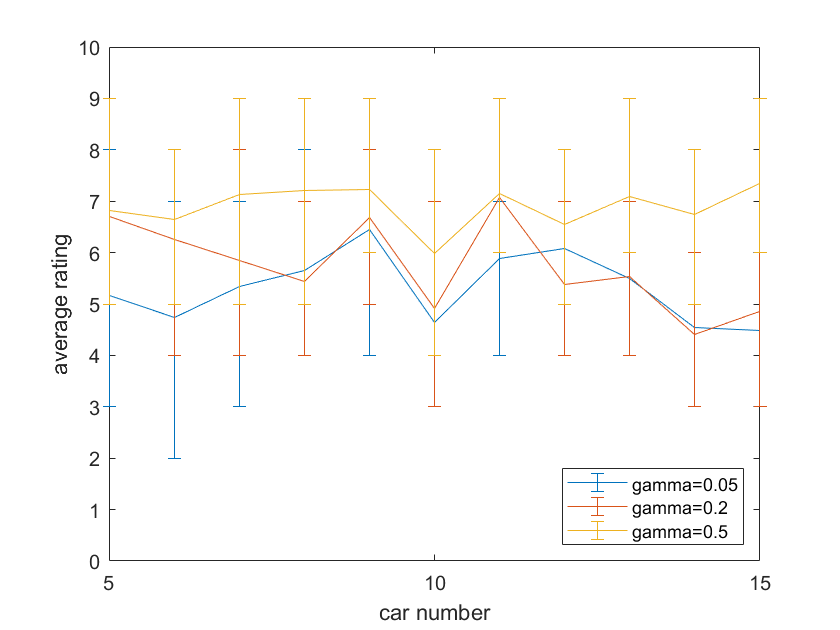
\includegraphics[width=0.49\linewidth]{figures/gamma_centerlo_err.png}}
  \caption{不同$\gamma$值在两种评价分布模式下对应的消息总评价均值与最值}
  \label{fig:gammaerr}
\end{figure}

从以上结果可以看到,消息总评价在统计学上整体向中心靠拢,但同时存在较大的波动空间,其具体结果还依具体情况而定。由于算法需要为信誉值确定一个判定消息是否可信的标准,依据消息总评价$Cred_m$划分可信区间如下:

\begin{equation*}
    \begin{aligned}
        &1\leq Cred_m\leq 5,\ \mbox{消息不可信,信誉值减小} \\
        &5< Cred_m\leq 6,\ \mbox{中立,信誉值不变} \\
        &6< Cred_m\leq 10,\ \mbox{消息可信,信誉值增加}
    \end{aligned}
\end{equation*}
写成公式:6-10:可信,信誉值增加;5-6:中立,信誉值不变;1-5:不可信,信誉值减小。

将消息评价的可信区间按此方式划分,是基于本节模拟实验的结果,考虑到完全随机的情况下评价均值统一趋近于5分,可以认为该分数对应着相对平均、难以判定正负的中立情况,而将中立区间设置得相对偏高,则是考虑到了对于不诚实消息传播者应当基于更严厉的评判标准。

\section{参数选取结果}

根据以上模拟测试与分析,确定信誉算法的相关参数为:

\begin{equation*}
    \begin{aligned}
        \delta&=0.2 \\
        \theta_{s}=2&,\ \theta_{f}=-3 \\
        \gamma=0.2,\ C_0&=5,\ C_1=6
    \end{aligned}
\end{equation*}

该组参数的选取确保了系统对于用户提交数据时间以及具体交互结果的敏感度,在智能合约进行小数截断的情况下,系统对每次交互都能产生较为明显的反馈;同时,尽量保证了在数据提交频繁的情况下,信誉值依然维持在合理的波动范围内,以避免在车辆极其密集的场景中,该评估结果由于产生极端的大幅波动而失去参考价值。该组参数在系统综合测试中的整体表现将在第5章中得到详细的描述与分析。

\section{本章小结}
本章利用原型系统设计了一系列实验,对信誉算法的参数取值进行了测试与分析。通过模拟实验,本章分别对算法中时间衰减系数、位置验证、消息传播几部分相关的参数进行了调优,从系统对时间和交互失败结果的敏感度、信誉整体走势、数据波动性等方面进行评价,并且最终确定了合适的参数值。


% 其他部分
\backmatter

% 参考文献
\bibliography{ref/refs}  % 参考文献使用 BibTeX 编译
% \printbibliography       % 参考文献使用 BibLaTeX 编译

% 附录
\appendix
% % !TeX root = ../thuthesis-example.tex

\begin{survey}
\label{cha:survey}

\title{Title of the Survey}
\maketitle


\tableofcontents


本科生的外文资料调研阅读报告。


\section{Figures and Tables}

\subsection{Figures}

An example figure in appendix (Figure~\ref{fig:appendix-survey-figure}).

\begin{figure}
  \centering
  
\includegraphics[width=0.6\linewidth]{example-image-a.pdf}
  \caption{Example figure in appendix}
  \label{fig:appendix-survey-figure}
\end{figure}


\subsection{Tables}

An example table in appendix (Table~\ref{tab:appendix-survey-table}).

\begin{table}
  \centering
  \caption{Example table in appendix}
  \begin{tabular}{ll}
    \toprule
    File name       & Description                                         \\
    \midrule
    thuthesis.dtx   & The source file including documentaion and comments \\
    thuthesis.cls   & The template file                                   \\
    thuthesis-*.bst & BibTeX styles                                       \\
    thuthesis-*.bbx & BibLaTeX styles for bibliographies                  \\
    thuthesis-*.cbx & BibLaTeX styles for citations                       \\
    \bottomrule
  \end{tabular}
  \label{tab:appendix-survey-table}
\end{table}


\section{Equations}

An example equation in appendix (Equation~\eqref{eq:appendix-survey-equation}).
\begin{equation}
  \frac{1}{2 \uppi \symup{i}} \int_\gamma f = \sum_{k=1}^m n(\gamma; a_k) \mathscr{R}(f; a_k)
  \label{eq:appendix-survey-equation}
\end{equation}


\section{Citations}

Example citations in appendix.
\cite{abrahams99tex}
\cite{salomon1995advanced}
\cite{abrahams99tex,salomon1995advanced}


\bibliographystyle{unsrtnat}
\bibliography{ref/appendix}

\end{survey}
       % 本科生:外文资料的调研阅读报告
% % !TeX root = ../thuthesis-example.tex

\begin{translation}
\label{cha:translation}

\title{书面翻译题目}
\maketitle

\tableofcontents


本科生的外文资料书面翻译。


\section{图表示例}

\subsection{图}

附录中的图片示例(图~\ref{fig:appendix-translation-figure})。

\begin{figure}
  \centering
  
\includegraphics[width=0.6\linewidth]{example-image-a.pdf}
  \caption{附录中的图片示例}
  \label{fig:appendix-translation-figure}
\end{figure}


\subsection{表格}

附录中的表格示例(表~\ref{tab:appendix-translation-table})。

\begin{table}
  \centering
  \caption{附录中的表格示例}
  \begin{tabular}{ll}
    \toprule
    文件名          & 描述                         \\
    \midrule
    thuthesis.dtx   & 模板的源文件,包括文档和注释 \\
    thuthesis.cls   & 模板文件                     \\
    thuthesis-*.bst & BibTeX 参考文献表样式文件    \\
    thuthesis-*.bbx & BibLaTeX 参考文献表样式文件  \\
    thuthesis-*.cbx & BibLaTeX 引用样式文件        \\
    \bottomrule
  \end{tabular}
  \label{tab:appendix-translation-table}
\end{table}


\section{数学公式}

附录中的数学公式示例(公式~\eqref{eq:appendix-translation-equation})。
\begin{equation}
  \frac{1}{2 \uppi \symup{i}} \int_\gamma f = \sum_{k=1}^m n(\gamma; a_k) \mathscr{R}(f; a_k)
  \label{eq:appendix-translation-equation}
\end{equation}


\section{文献引用}

文献引用示例\cite{abrahams99tex}。


% 书面翻译的参考文献
\bibliographystyle{unsrtnat}
\bibliography{ref/appendix}

% 书面翻译对应的原文索引
\begin{translation-index}
  \nocite{salomon1995advanced}
  \bibliographystyle{unsrtnat}
  \bibliography{ref/appendix}
\end{translation-index}

\end{translation}
  % 本科生:外文资料的书面翻译
% !TeX root = ../thuthesis-example.tex

\chapter{补充内容}

附录是与论文内容密切相关、但编入正文又影响整篇论文编排的条理和逻辑性的资料,例如某些重要的数据表格、计算程序、统计表等,是论文主体的补充内容,可根据需要设置。


\section{图表示例}

\subsection{图}

附录中的图片示例(图~\ref{fig:appendix-figure})。

\begin{figure}
  \centering
  
\includegraphics[width=0.6\linewidth]{example-image-a.pdf}
  \caption{附录中的图片示例}
  \label{fig:appendix-figure}
\end{figure}


\subsection{表格}

附录中的表格示例(表~\ref{tab:appendix-table})。

\begin{table}
  \centering
  \caption{附录中的表格示例}
  \begin{tabular}{ll}
    \toprule
    文件名          & 描述                         \\
    \midrule
    thuthesis.dtx   & 模板的源文件,包括文档和注释 \\
    thuthesis.cls   & 模板文件                     \\
    thuthesis-*.bst & BibTeX 参考文献表样式文件    \\
    thuthesis-*.bbx & BibLaTeX 参考文献表样式文件  \\
    thuthesis-*.cbx & BibLaTeX 引用样式文件        \\
    \bottomrule
  \end{tabular}
  \label{tab:appendix-table}
\end{table}


\section{数学公式}

附录中的数学公式示例(公式~\eqref{eq:appendix-equation})。
\begin{equation}
  \frac{1}{2 \uppi \symup{i}} \int_\gamma f = \sum_{k=1}^m n(\gamma; a_k) \mathscr{R}(f; a_k)
  \label{eq:appendix-equation}
\end{equation}


% 致谢
% !TeX root = ../thuthesis-example.tex

\begin{acknowledgements}
谨向清华大学计算机系的向勇副教授表示衷心的感谢。在完成论文相关工作的过程中,老师对我进行了悉心的指导,从研究内容到日常生活,从知识学习、创新实践到进度安排、习惯养成,老师给予了我很多建议与帮助,使我在这一学期的时间里得到了全面的提升与成长。同时,感谢实验室全体老师与同学在研究期间对我的支持,在我遇到困难时能够第一时间为我提供协助,对我的工作提出了许多宝贵的改进意见。

感谢母校成就了我充实而精彩的四年大学生活。在这里,我享受到了便利的生活环境、优秀的课程资源,各位老师的言传身教使我受益匪浅,同学之间的深厚情谊我也将铭记在心。在这里,我曾在训练场上接受过烈日的炙烤,在宿舍中厅挑灯夜战后见证过冬日的第一缕晨光,当然也曾在雨中与三两好友漫步谈心,在夜晚为一段工作的结束和众人共同欢庆。感谢所有与我一同经历这些瞬间的人们,与你们每一位的相遇共同塑造了今天的我自己。

最后,感谢我的父母家人。到现在为止,他们陪伴我的时间是我整个大学时光的五倍,在这段时间里他们对我无条件的关爱、包容与支持从未改变,我对他们的感激之情难以用文字充分表达,只期望在更加漫长的时光中用自己的行动去书写。

论文写到这里就要结束了,正如自己四年的大学时光,在弹指间也接近了尾声。回顾过去,自己的生活很难说充满了诗意或伟大的时刻,但总归是踏实而惬意的;正如这篇致谢,不为花哨,只希望能真挚、诚恳地表达出自己的一点心情。
\end{acknowledgements}


% 声明
\statement
% 生成的声明页是否要插入页眉和页脚(默认 empty)
% 仅在需要进行电子签名时,才需要打开这一选项
% 插入的扫描声明页总是会生成页眉(研究生)和页脚,不受这一选项影响
% \statement[page-style=plain]
% 将签字扫描后的声明文件 scan-statement.pdf 替换原始页面
% \statement[file=scan-statement.pdf]

% 个人简历、在学期间完成的相关学术成果
% !TeX root = ../thuthesis-example.tex

\begin{resume}

  \section*{个人简历}

  197× 年 ×× 月 ×× 日出生于四川××县。

  1992 年 9 月考入××大学化学系××化学专业,1996 年 7 月本科毕业并获得理学学士学位。

  1996 年 9 月免试进入清华大学化学系攻读××化学博士至今。


  \section*{在学期间完成的相关学术成果}

  \subsection*{学术论文}

  \begin{achievements}
    \item Yang Y, Ren T L, Zhang L T, et al. Miniature microphone with silicon-based ferroelectric thin films[J]. Integrated Ferroelectrics, 2003, 52:229-235.
    \item 杨轶, 张宁欣, 任天令, 等. 硅基铁电微声学器件中薄膜残余应力的研究[J]. 中国机械工程, 2005, 16(14):1289-1291.
    \item 杨轶, 张宁欣, 任天令, 等. 集成铁电器件中的关键工艺研究[J]. 仪器仪表学报, 2003, 24(S4):192-193.
    \item Yang Y, Ren T L, Zhu Y P, et al. PMUTs for handwriting recognition. In press[J]. (已被Integrated Ferroelectrics录用)
  \end{achievements}


  \subsection*{专利}

  \begin{achievements}
    \item 任天令, 杨轶, 朱一平, 等. 硅基铁电微声学传感器畴极化区域控制和电极连接的方法: 中国, CN1602118A[P]. 2005-03-30.
    \item Ren T L, Yang Y, Zhu Y P, et al. Piezoelectric micro acoustic sensor based on ferroelectric materials: USA, No.11/215, 102[P]. (美国发明专利申请号.)
  \end{achievements}

\end{resume}


% 指导教师/指导小组学术评语
% !TeX root = ../thuthesis-example.tex

\begin{comments}
% \begin{comments}[name = {指导小组学术评语}]
% \begin{comments}[name = {Comments from Thesis Supervisor}]
% \begin{comments}[name = {Comments from Thesis Supervision Committee}]


\end{comments}


% 答辩委员会决议书
% !TeX root = ../thuthesis-example.tex

\begin{resolution}

\end{resolution}


% 本科生的综合论文训练记录表(扫描版)
% \record{file=scan-record.pdf}

\end{document}
